\documentclass[a4paper,11pt]{article}
\pdfoutput=1 % if your are submitting a pdflatex (i.e. if you have
             % images in pdf, png or jpg format)

\usepackage{jcappub}
\usepackage{graphicx}
\usepackage{dcolumn}
\usepackage{amssymb,amsmath,bm}
\usepackage{color}
\usepackage[dvipsnames]{xcolor}
%\usepackage[colorlinks,linkcolor=red,citecolor=blue,urlcolor=blue ]{hyperref}
\usepackage[utf8]{inputenc}
\usepackage{lipsum}
\usepackage{xfrac}
\usepackage{aas_macros}
\usepackage{mathrsfs}
\usepackage{subfigure}
\newcommand{\nv}{\vec{\theta}}
%\newcommand{\pasj}{Publications of the ASJ}
%\newcommand{\aap}{Astronomy and Astrophysics}
%\newcommand{\apj}{Astrophysical Journal}
%\newcommand{\apjs}{Astrophysical Journal, Supplement}
%\newcommand{\mnras}{Monthly Notices of the RAS}
\newcommand{\todo}[1]{{\bf TODO: #1}}

\newcommand{\as}[1]{{\textcolor{blue}{[AS: #1]}}}
\newcommand{\an}[1]{{\textcolor{magenta}{[AN: #1]}}}

\newcommand\Tstrut{\rule{0pt}{3ex}}   

\usepackage[T1]{fontenc} % if needed
\usepackage{natbib}
\bibliographystyle{JHEP}
\title{Tomographic galaxy clustering with the Subaru Hyper Suprime-Cam first year public data release}

\author[a,1]{Irst F.}
\author[b]{Econd S.}

\affiliation[a]{Dept. of Paranormal Activity, Miskatonic University, Arkham, MA}
\affiliation[b]{Some other place}
\emailAdd{irst.f@physics.msk.edu}

\abstract{ We analyze the clustering of galaxies in the first year public release of the Hyper Suprimer-Cam data. Despite the relatively small footprints of the observed fields, the data are an excellent model for the very deep future photometric datasets such as LSST. We analyze the sample split into four tomographic redshift bins centered at $z=0.4,0.6\ldots$. We measure the auto and cross-correlations between all bins and find a good fit to the data on scales $k\lesssim 0.8 h$/Mpc using a halo model with no evidence for systematics errors. Our six parameter model is consistent with galaxy sample being dominated by central galaxies living in halos of mass $\log M/M_\odot \gtrsim 10 + 4(1+z)^{-1}$.  While we project out systematic templates in the power spectrum measurement we find that they do not appreciably change the results. \as{Is this true for cross-correlations?}. We find that cross-correlations strongly constrain the difference between the effective tomographic redshifts, but the data is strongly degenerate with respect to  coherent shifts in redshift.
We test for magnification bias effect and constrain the lensing amplitude $A_L=3\pm 1$ consistent with standard lensing. 
}

\begin{document}
\maketitle
\flushbottom

\section{Introduction}\label{sec:intro}
\lipsum[1]

\section{Theory}\label{sec:theory}
  \subsection{Projected quantities and power spectra}\label{ssec:theory.cellpk}
    \todo{cites everywhere}
    Our main observable is the projected overdensity of galaxies $\delta^i_g(\nv)$ as a function of sky position $\nv$ in a given redshift bin labelled by $i$. This is related to the 3D galaxy overdensity $\Delta_g$ through
    \begin{equation}
      \delta^i_g(\nv)=\int dz\,p^i(z)\,\Delta_g\left(t(z),\chi(z)\nv\right).
    \end{equation}
    Here $t(z)$ and $\chi(z)$ are the cosmic time and radial comoving distance as a function of redshift, and $p^i(z)$ is the redshift bin window function, given by the true redshift distribution of objects in the bin normalized to unit area.
  
    Given the small size of the sky patches covered by the HSC DR1, we will adopt the flat sky approximation for simplicity, in which case $\nv$ is a 2D vector. It is common to decompose $\delta^i_g(\nv)$ into its Fourier coefficients
    \begin{equation}
      a^i_{\bf l}\equiv \int\frac{d\theta^2}{2\pi}e^{-i{\bf l}\cdot\nv}\delta^i_g(\nv).
    \end{equation}
    The variance of the Fourier coefficients is the so-called angular power spectrum $\langle a^i_{\bf l}a^{j*}_{{\bf l}'}\rangle = C^{ij}_\ell\,\delta^{\cal D}({\bf l}-{\bf l}')$, where $\delta^{\cal D}$ is the 2D Dirac delta function. The 3D power spectrum $P_{gg}(z,{\bf k})$ is defined analogously for the 3D Fourier coefficients of $\Delta_g$. Both quantities are related to each other through:
    \begin{equation}\label{eq:cell_gg_limber}
      C^{ij}_\ell = \int dz\,\frac{H(z)}{\chi^2(z)} p^i(z)p^j(z)\,P_{gg}\left(z,k=\frac{\ell+1/2}{\chi(z)}\right),
    \end{equation}
    where $H(z)$ is the expansion rate at redshift $z$, and we have used the so-called Limber approximation.
  
  \subsection{Magnification bias}\label{ssec:theory.mag}
    \todo{cites everywhere}
    Gravitational lensing alters the observed galaxy fluxes and distorts their observed positions. The combined effect, is a position-dependent modulation of the number density that distorts the clustering pattern.
    In the presence of this effect, the equations in the previous section get slightly modified. The projected galaxy overdensity becomes:
    \begin{equation}
      \delta^i_g(\nv)=\int dz\,\left[p^i(z)\,\Delta_g+\frac{W_\mu^i(z)}{H(z)}\nabla_\theta^2\nabla^{-2}\Delta_m\right],
    \end{equation}
    where $\Delta_m$ is the 3D matter overdensity (we have omitted the dependence on $t$ and $\chi\nv$ for brevity) and $W_\mu$ is the magnification kernel
    \begin{equation}
      W_\mu(z)=\frac{3H_0^2\Omega_M(1+z)}{2}\int_z^\infty dz'\,p^i(z)\,\left(5s(z')-2\right)\,\frac{\chi(z')-\chi(z)}{\chi(z)\chi(z')}.
    \end{equation}
    Here, $H_0\equiv H(z=0)$, $\Omega_M$ is the cosmological matter fraction, and $s$ is the logarithmic slope of the cumulative apparent magnitude distribution:
    \begin{equation}
      s(z) \equiv \frac{\partial \log_{10}N(<m, z)}{\partial m}.
      \label{eq:s-func}
    \end{equation}
    The angular power spectrum is then given by:
    \begin{equation}\label{eq:cell_gg_wmag}
      C^{ij}_\ell = \int dz\,\frac{H(z)}{\chi^2(z)}\left[p^ip^j\,P_{gg}+\left(p^iW_\mu^j+p^jW_\mu^i\right)\frac{\ell(\ell+1)}{Hk^2}P_{gm}+W_\mu^iW_\mu^j\left(\frac{\ell(\ell+1)}{Hk^2}\right)^2P_{mm}\right],
    \end{equation}
    where $P_{mm}$ is the 3D power spectrum of matter fluctuations, $P_{gm}$ is the galaxy-matter cross-spectrum and we have omitted the dependence of all quantities on $z$ or $k=(\ell+1/2)/\chi$ for brevity.

  \subsection{Halo Occupation Distribution}\label{ssec:theory.hod}
    In order to model $P_{gg}(z,k)$ we use a halo occupation distribution (HOD) model \todo{cites everywhere}. In this halo model-based presciption we model the galaxy content of dark matter haloes as a function of halo mass. Details about HOD parametrizations can be found in \todo{cite}. In short, the galaxy power spectrum receives contributions from the so-called 1-halo and 2-halo terms:
    \begin{equation}
      P_{gg}(z,k) = P_{gg,{\rm 1h}}(z,k) + P_{gg,{\rm 2h}}(z,k),
    \end{equation}
    where
    \begin{align}
      & P_{gg,{\rm 1h}}(k)=\frac{1}{\bar{n}_g^2} \int dM\,\frac{dn}{dM} \bar{N}_c\,\left[\bar{N}_s^2u_s^2(k)+2\bar{N}_su_s^2(k)\right],\\
      & P_{gg,{\rm 2h}}(k)=\left(\frac{1}{\bar{n}_g} \int dM\,\frac{dn}{dM}\,b_h(M)\,\bar{N}_c\,\left[1+\bar{N}_su_s(k)\right]\right)^2\,P_{\rm lin}(k).
    \end{align}
    Here, $M$ represents halo mass, $dn/dM$ is the halo mass function, $b_h(M)$ is the halo bias, $\bar{N}_c(M)$ and $\bar{N}_s(M)$ are the mean number of central and satellite galaxies respectively, $u_s(k)$ is the Fourier transform of the normalized density profile of satellite galaxies, $P_{\rm lin}(k)$ is the linear matter power spectrum and $\bar{n}_g$ is the total mean galaxy density, given by
    \begin{equation}
      \bar{n}_g=\int dM\,\frac{dn}{dM}\bar{N}_c(M)\left[1+\bar{N}_s(M)\right].
    \end{equation}
    A central assumption in standard HOD parametrizations is that centrals/satellites follow a binomial/Poisson distribution.

    Following \todo{cite}, we parametrise the number of centrals and satellites as a function of mass as:
    \begin{align}
      &\bar{N}_c(M)=\frac{1}{2}\left[1+{\rm erf}\left(\frac{\log(M/M_{\rm min})}{\sigma_{{\rm ln}M}}\right)\right],\\
      &\bar{N}_s(M)=\Theta(M-M_0)\left(\frac{M-M_0}{M_1'}\right)^\alpha,
    \end{align}
    where $\Theta(x)$ is the Heavyside step function. Furthermore, we assume that $N_c$ follows a Bernoulli distribution with probability $p=\bar{N}_c$, and that the number of satellites is Poisson-distributed with mean $\bar{N}_s$. Finally, we model the distribution of satellites to follow that of the dark matter, and therefore $u_s$ is a Navarro-Frenk-White profile, given by:
    \begin{equation}
      u_s(k|M)=\frac{\sin x\left[{\rm Si}\left((1+c)\,x\right)-{\rm Si}(x)\right]+\cos x\left[{\rm Ci}\left((1+c)x\right)-{\rm Ci}(x)\right]-\frac{\sin(cx)}{(1+c)x}}{{\rm ln}(1+c)-\frac{c}{1+c}},
    \end{equation}
    where $x=k R_\Delta/c$, $R_\Delta$ is the halo radius, $c=c(M)$ is the concentration parameter, and ${\rm Si}/{\rm Ci}$ are the sine and cosine integral functions. We define $R_\Delta$ as the radius that encloses $\Delta=200$ times the background matter density. The concentration-mass relation $c(M)$ also depends on the choice of $\Delta$, and we follow the parametrization of Duffy et al. \todo{cite}.

    In order to include lensing magnification in the theory prediction, we also need to model the galaxy-matter and matter-matter power spectra (see Eq. \ref{eq:cell_gg_wmag}). Following the HOD parametrization, the 1-halo and 2-halo contributions to $P_{gm}(k)$ are given by:
    \begin{align}
      & P_{gm,{\rm 1h}}(k)=\frac{1}{\bar{n}_g\bar{\rho}_M} \int dM\,\frac{dn}{dM} M\,\bar{N}_c\,\left[1+\bar{N}_su_s(k)\right],\\
      & P_{gm,{\rm 2h}}(k)=\left(\frac{1}{\bar{n}_g} \int dM\,\frac{dn}{dM}\,b_h(M)\,\bar{N}_c\,\left[1+\bar{N}_su_s(k)\right]\right)\,P_{\rm lin}(k),
    \end{align}
    where $\bar{\rho}_M$ is the comoving matter density. $P_{mm}(k)$ is simply given by the {\tt Halofit} parametrization of \todo{cite}.

    It is a well-known fact that the simple halo model implementation described here is not able to accurately describe the ``quasi-linear'' scales in the transition between the 1-halo and 2-halo-dominated regimes, corresponding to $k\sim0.1\,{\rm Mpc}^{-1}$ at $z\sim0$ \todo{cite}. To correct for this inaccuracy, we simply multiply $P_{gg}$ and $P_{gm}$ by a universal scale-dependent factor, given by the ratio between the {\tt Halofit} and the pure halo model predictions for $P_{mm}$:
    \begin{equation}
      R(z,k)=\frac{P^{\rm Halofit}_{mm}(z,k)}{P^{\rm halo\,model}_{mm}(z,k)}.
    \end{equation}
    
We expect mean galaxy properties to evolve as a function of redshift for the magnitude-limited sample considered in this analysis. Instead of fitting a separate HOD model to each redshift bin, we fit redshift-dependent functions to $M_{\mathrm{min}}$, $M_{0}$ and $M_{1}$ and choose a functional form given by:
\begin{equation}
M_{i}(z) = M_{i} + M_{i, p} \left(\frac{1}{1+z} - \frac{1}{1+z_{p}}\right),
\end{equation}
where $i \in [\mathrm{min}, 0, 1]$ and $z_{p}$ denotes a pivot redshift, which we set to $z_{p} = 0.65$. This functional form is motivated by an initial analysis in which we separately fit an HOD to each auto-power spectrum and determine a function consistent with the observed redshift evolution of the three parameters $M_{\mathrm{min}}$, $M_{0}$ and $M_{1}$. We additionally include a pivot redshift $z_{p}$ in our parametrization to remove degeneracies between the fitted parameters. 


\section{Data}\label{sec:data}
  \begin{table}
  \centering
  \begin{tabular}{|l|l|}
  \hline
   {\bf Cut} & {\bf Comment} \\
   \hline
   \texttt{detect\_is\_primary}=True & Basic quality cuts, \\
   \texttt{icmodel\_flags\_badcentroid}=False & see \cite{2018PASJ...70S..25M,2018PASJ...70S...5B}\\
   \texttt{icentroid\_sdss\_flags}=False & \\
   \texttt{iflags\_pixel\_edge}=False & \\
   \texttt{iflags\_pixel\_interpolated\_center}=False & \\
   \texttt{iflags\_pixel\_saturated\_center}=False & \\
   \texttt{iflags\_pixel\_cr\_center}=False & \\
   \texttt{iflags\_pixel\_bad}=False & \\
   \texttt{iflags\_pixel\_suspect\_center}=False & \\
   \texttt{iflags\_pixel\_clipped\_any}=False & \\
   \texttt{meas.ideblend\_skipped}=False & \\
   \texttt{iblendedness\_abs\_flux}$<10^{-0.375}$ & \\
   \hline % Strict from here on
   \texttt{[g,r,z,y]centroid\_sdss\_flags}=False & Strict photometry cuts\\
   \texttt{[g,r,i,z,y]cmodel\_flux\_flags}=False & \\
   \texttt{[g,r,i,z,y]flux\_psf\_flags}=False & \\
   \texttt{[g,r,z,y]flags\_pixel\_edge}=False & \\
   \texttt{[g,r,z,y]flags\_pixel\_interpolated\_center}=False & \\
   \texttt{[g,r,z,y]flags\_pixel\_saturated\_center}=False & \\
   \texttt{[g,r,z,y]flags\_pixel\_cr\_center}=False & \\
   \texttt{[g,r,z,y]flags\_pixel\_bad}=False & \\
   \hline
   \texttt{icmodel\_mag}$-$\texttt{a\_i} $<$ 24.5 & Magnitude limit\\ % Magnitude cut
   \hline
   \texttt{icmodel\_flux}$>10\,$\texttt{icmodel\_flux\_err} & 10$\sigma$ detections\\
   \hline
   \texttt{[g,r,y,z]cmodel\_flux}$>5\,$\texttt{[g,r,y,z]cmodel\_flux\_err} & 5$\sigma$ detection  (required \\
   & only in 2 other bands)\\
   \hline
   \texttt{iclassification\_extendedness}=1 & Star-galaxy separator\\
   \hline
  \end{tabular}
  \caption{Summary of the selection cuts performed to the original dataset to retrieve the sample considered in our analysis.} \label{tab:cuts_summary}
  \end{table}  

  \begin{table}
  \centering
  \begin{tabular}{|l|r|c|l|}
   \hline
   {\bf Field name} & $N_{\rm gal}$ & {\bf Area} (deg$^2$) & $f_{\rm sky}$ \\
   \hline
   GAMA09H  & 1,697,713 & 14.5 & $3.5\times10^{-4}$ \\
   GAMA15H  & 1,695,364 & 15.1 & $3.7\times10^{-4}$ \\
   HECTOMAP &   639,970 &  5.1 & $1.2\times10^{-4}$ \\
   VVDS     & 2,340,965 & 20.6 & $5.0\times10^{-4}$ \\
   WIDE12H  & 1,220,816 & 11.6 & $2.8\times10^{-4}$ \\
   XMMLSS   & 2,139,629 & 20.8 & $5.0\times10^{-4}$ \\
   \hline
   Total    & 9734457 & 87.7 & $2.1\times10^{-3}$ \\
   \hline
  \end{tabular}
  \caption{Summary of the 6 different fields used in our analysis. The second column lists the number of galaxies in the DR1 catalog passing the cuts in Table \ref{tab:cuts_summary}. The third and fourth columns show the area and corresponding sky fraction covered by each field. The area was calculated as the sum of pixel areas allowed by the sky mask described in Section \ref{ssec:methods.mask}.} \label{tab:field_summary}
  \end{table}  

  \begin{table}
  \centering
  \begin{tabular}{|l|l|l|l|}
    \hline
    $z_{\rm phot}^{\rm ini}$ & $z_{\rm phot}^{\rm end}$ & $\bar{z}$ & $N_{\rm gal}$ \\
    \hline
    0.15 & 0.5  & 0.57 & 1,750,274 \\
    0.5  & 0.75 & 0.68 & 1,766,939 \\
    0.75 & 1.0  & 0.91 & 1,702,685 \\
    1.0  & 1.5  & 1.26 & 1,752,359 \\
    \hline
  \end{tabular}
  \caption{Summary of the 4 redshift bins used in our analysis. The first two columns show the photo-$z$ bin edges. We used the {\tt photoz\_best} redshift estimator for the photo-$z$ code {\tt ephor\_ab} to assign galaxies to different bins. The second column shows the mean redshift of each bin calculated from the fiducial redshift distributions described in Section \ref{ssec:methods.nz}. The last column shows the number of galaxies in each bin. The bin edges were chosen to roughly contain an equal number of galaxies in each of them.} \label{tab:bins_summary}
  \end{table}
  
  We use data from the Hyper Suprime-Cam Subaru Strategic Program first data release (HSC DR1 hereon)\footnote{https://hsc-release.mtk.nao.ac.jp}. The release is extensively documented in \cite{2018PASJ...70S...8A}, and we only provide the details of the galaxy sample and associated data used for our clustering analysis.
  
  \todo{General blurb about HSC DR1}
  
  We use a magnitude-limited sample constructed from the WIDE DR1 sample by imposing data cuts that are similar to those used to create the HSC shear catalog \cite{2018PASJ...70S..25M}. The exact cuts are shown in Table~\ref{tab:cuts_summary}, and can be summarized as follows: besides a minimal set of quality cuts (selecting only primary detections with well-measured fluxes in all bands, removing objects near bad pixels, deblender artifacts, etc.), we impose an overall apparent magnitude cut in the extinction-corrected band $i_{\rm corr}<24.5$. This choice was based on a study of the survey depth-completeness relation in order to select a homogeneous and complete sample of high-confidence ($>10\sigma$) detections (see Section \ref{ssec:methods.syst}). We also select only objects with significant detections ($>5\sigma$) in at least two of the 4 remaining bands ($g,\,r,\,z,\,y$), and remove all objects classified as stars by the data reduction pipeline, using the "extendedness`` classifier as described in \cite{2018PASJ...70S..25M,2018PASJ...70S...5B}. The resulting sample has 9,734,457 objects and covers $\sim88$ square degress distributed across the 6 HSC DR1 fields described in Table \ref{tab:field_summary}.

  All objects have photometric redshift measurements from 6 different codes as presented in \cite{2018PASJ...70S...9T}. We use the {\tt photoz\_best} redshift estimator assigned by the {\tt ephor\_ab} method as a marker to divide the sample into 4 redshift bins containing roughly equal numbers of galaxies. The {\tt photoz\_best} estimator is defined to minimize the risk that the true galaxy redshift lie outside the range $z_{\rm true}\pm 0.15(1+z_{\rm true})$, where $z_{\rm true}$ is the galaxie's true redshift. A peliminary Fisher matrix study showed that the information content saturates quickly when slicing the data into finer redshift bins. The redshift bins are described in Table \ref{tab:bins_summary}, and the associated redshift distributions are discussed in Section \ref{ssec:methods.nz}.

\section{Methods}\label{sec:methods}
  The following sections describe the methods used to construct the data vector of angular power spectra and its covariance matrix used to constrain the parameters of our model.
  
  \subsection{Pixels and maps}\label{ssec:methods.pix}
    Our $C_\ell$-based analysis requires us to make maps of different quantities. The HSC DR1 is distributed across the 6 small ($\lesssim20\,{\rm deg.}^2$) fields summarized in Table \ref{tab:field_summary}. In this case, storing maps covering the full sky down to arcminute resolution, and performing operations on them such as spherical harmonic transforms, would be computationally inefficient and unnecessary. Instead, we perform separate power spectrum measurements on each individual field, with maps defined on rectangular sky patches covering them. Furthermore, the small size of each field allows us to make use of the flat-sky approximation safely. This leads to additional gains in speed, since spherical harmonic transforms can be replaced by the far more efficient fast Fourier transforms (FFTs).
    
    To generate maps of all the quantities described in this section we make use of a rectangular pixelization scheme using the Plate Carr\'ee projection (labelled {\tt CAR} in the World Coordinate System standard \cite{2002A&A...395.1077C}). In this case, pixels are simply defined by equal intervals of colatitude $\theta$ and azimuth $\phi$. To minimize the distortions caused by the flat-sky approximation, we place the projection reference point (i.e. a point in the equator $\theta=\pi/2$) at the center of each field. We use square pixels of size $\alpha_{\rm pix}=0.6'$ on a side, corresponding to a Nyquist frequency $\ell_{\rm Nyquist}=18,000$. The maps are defined on a rectangular patch large enough to cover all objects in each field, leaving a buffer of 10 masked pixels on all edges to avoid boundary effects on the FFTs.
  
  \subsection{Survey mask}\label{ssec:methods.mask}
    \begin{figure}
      \centering
      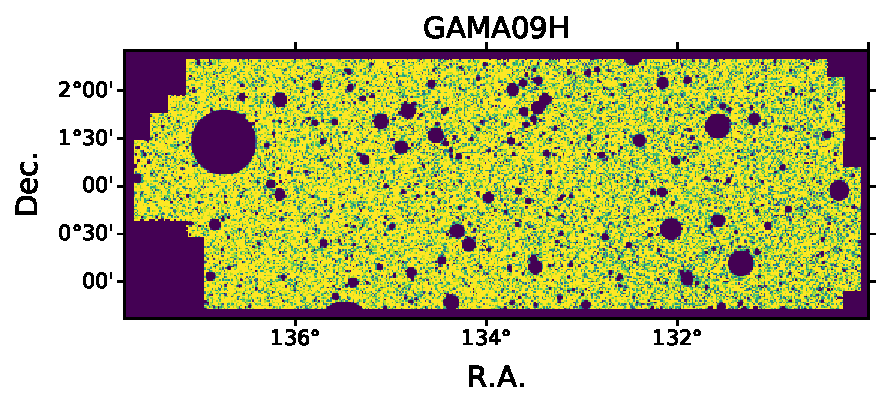
\includegraphics[width=0.49\textwidth]{figures/mask_GAMA09H.pdf}
      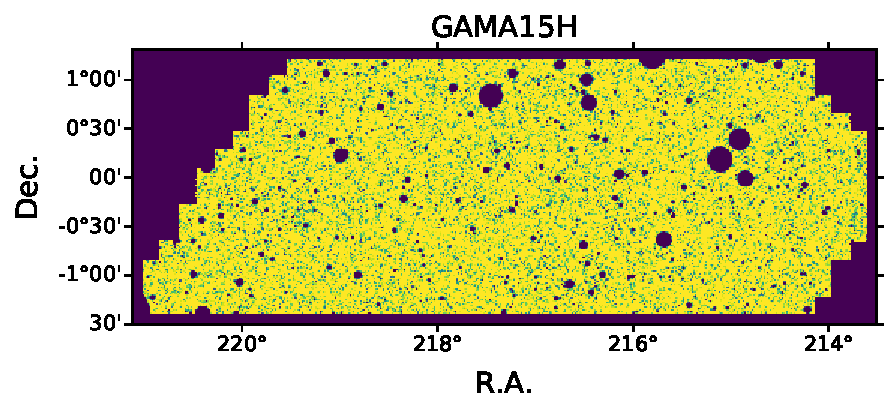
\includegraphics[width=0.49\textwidth]{figures/mask_GAMA15H.pdf}
      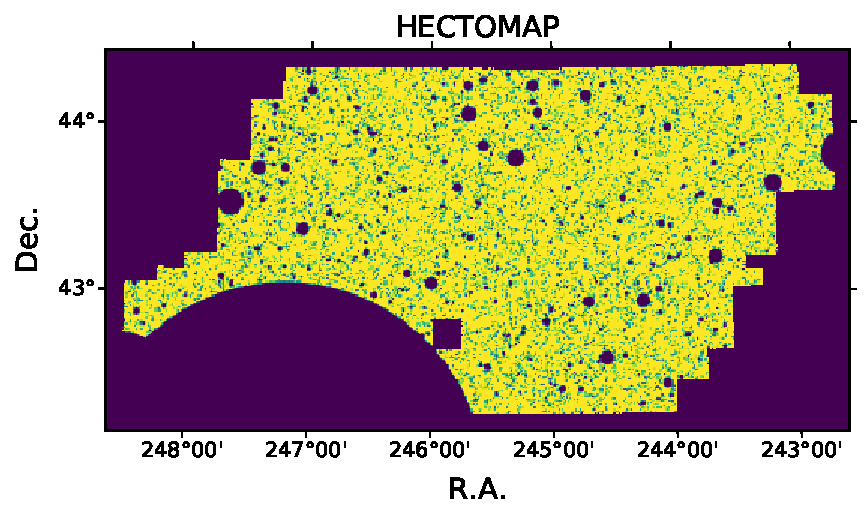
\includegraphics[width=0.49\textwidth]{figures/mask_HECTOMAP.pdf}
      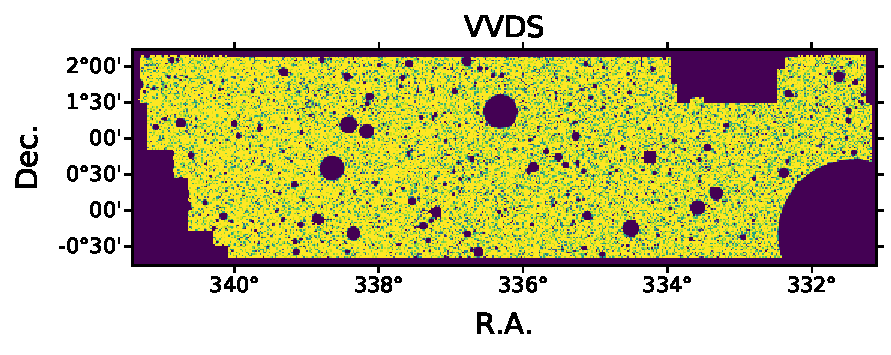
\includegraphics[width=0.49\textwidth]{figures/mask_VVDS.pdf}
      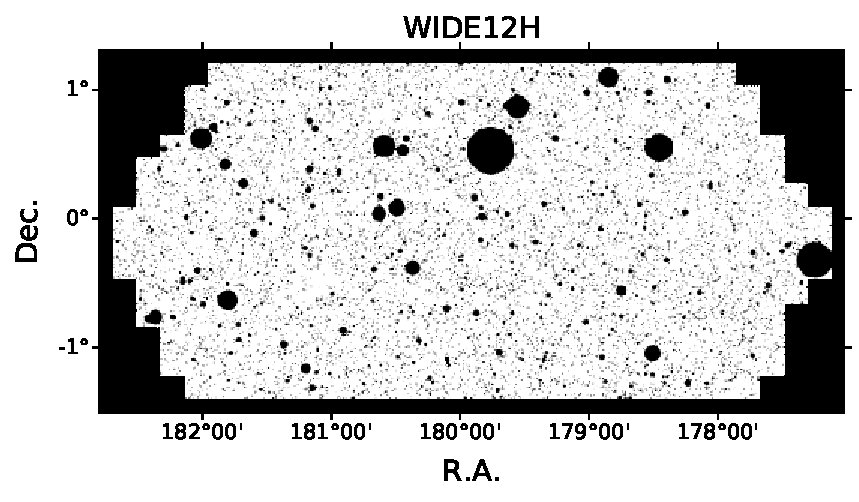
\includegraphics[width=0.49\textwidth]{figures/mask_WIDE12H.pdf}
      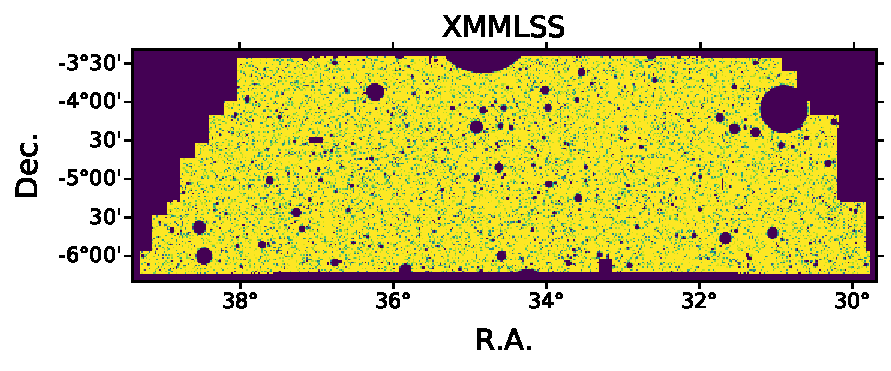
\includegraphics[width=0.49\textwidth]{figures/mask_XMMLSS.pdf}
      \caption{Sky masks for the 6 fields used in this analysis. The map pixels contain values between 0 and 1, corresponding to the fraction of the pixel's area not covered by the fiducial bright-object mask.}
      \label{fig:masks}
    \end{figure}
    The reconstruction of the survey geometry is a central step in order to obtain unbiased estimates of the angular power spectrum. This information is encoded in the so-called ``survey mask'', which minimally encodes binary information about which areas of the sky should (mask$=1$) or should not (mask$=0$) be used in the analysis. The basis for our survey mask is the so-called ``bright-object mask'' \cite{2018PASJ...70S...7C}, provided with the HSC DR1, which flags sources that are close to bright stars (mag $<17.5$), with a magnitude-dependent exclusion radius (see \cite{2018PASJ...70S...7C} for details). It is worth noting that the information about the bright object mask is encoded in the HSC DR1 at the catalog level in terms of per-object flags. We transform this information into a pixelized sky map through a multi-step process:
    \begin{enumerate}
      \item We start by creating a low-resolution binary mask based on the presence of objects from the raw catalog in a given pixel. This mask has a pixel size of 0.6 arcmin. The large number density of the raw catalog  ($n_g\sim30\,{\rm arcmin}^{-2}$) is high enough that masked pixels are unlikely to corresponds to intrinsically empty regions of the sky, but rather completely unobserved pixels.
      \item We upgrade the low-resolution binary mask to a higher resolution (0.2 arcmin), and remove all pixels containing objects flagged by the bright object mask. We then remove all disconnected, unmasked group of pixels, corresponding to spurious islands within the exclusion radius of a bright object with no sources in the catalogs.
      \item We downgrade the resulting mask back to the original resolution through an averaging procedure, producing a map quantifying the observed fraction of each pixel.
    \end{enumerate}
    It is worth noting that the resolution of the resulting mask ($0.6$ arcminutes) defines the resolution of all maps used in this analysis. After this procedure, we further mask all pixels with a $10\sigma$ depth below our magnitude limit of $i<24.5$, where the depth is estimated as described in Section \ref{ssec:methods.syst}.
    
    This defines our fiducial masks, which are shown in Figure \ref{fig:masks} for each field. As part of our systematics analysis (see Section \todo{reference}), we also study the effect of masking regions with significant contamination from the different observing conditions (described in Section \ref{ssec:methods.syst}) dependence of our measurements. It is worth noting that the NOMAD star catalog \cite{2004AAS...205.4815Z}, one of the datasets used to construct the brigh-object mask described above, is contaminated by a small fraction of bright nearby galaxies ($\sim10\%$). To study the impact of this contamination on our clustering measurements, we have also estimated the angular power spectra using a more recent version of the star mask (the so-called ``Arcturus'' mask described in \cite{2018PASJ...70S...7C}).

  \subsection{Systematics maps}\label{ssec:methods.syst}
    \begin{figure}
      \centering
      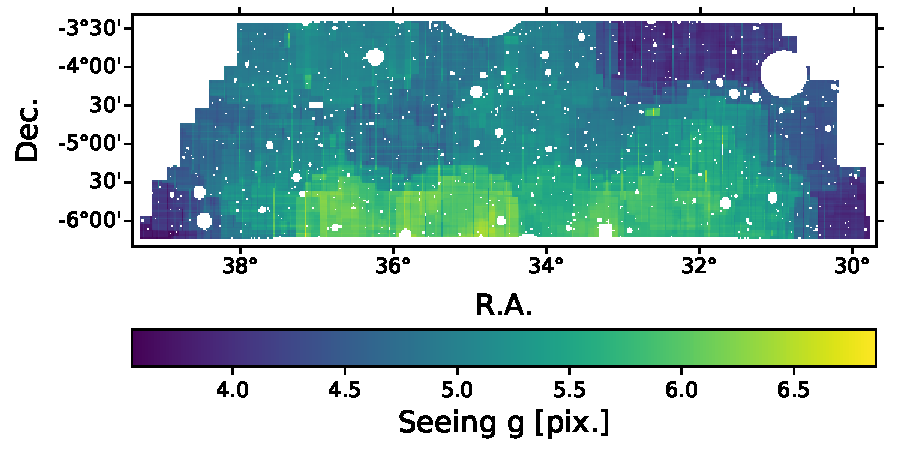
\includegraphics[width=0.49\textwidth]{figures/syst_seeing_g.pdf}
      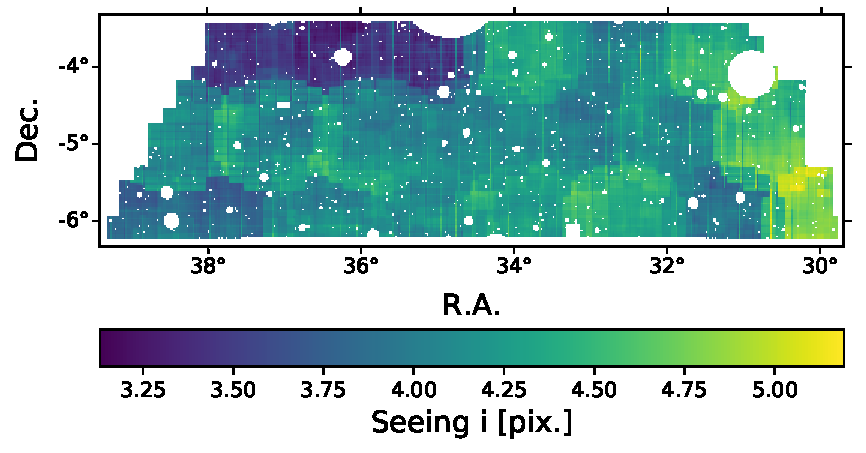
\includegraphics[width=0.49\textwidth]{figures/syst_seeing_i.pdf}
      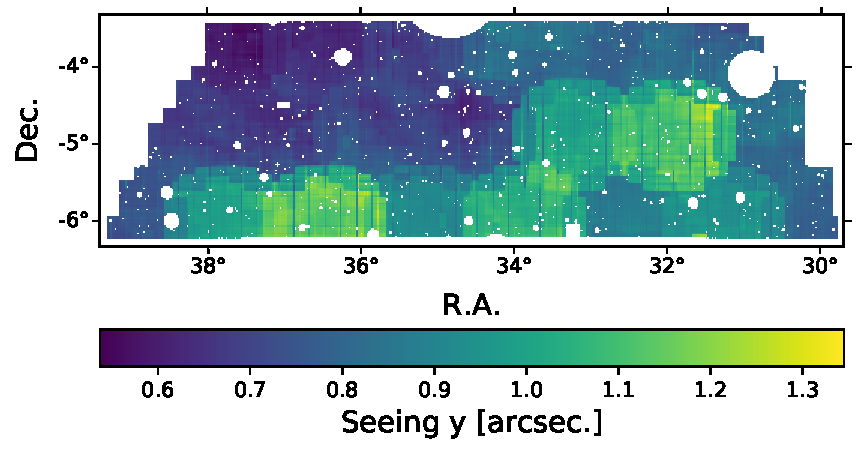
\includegraphics[width=0.49\textwidth]{figures/syst_seeing_y.pdf}
      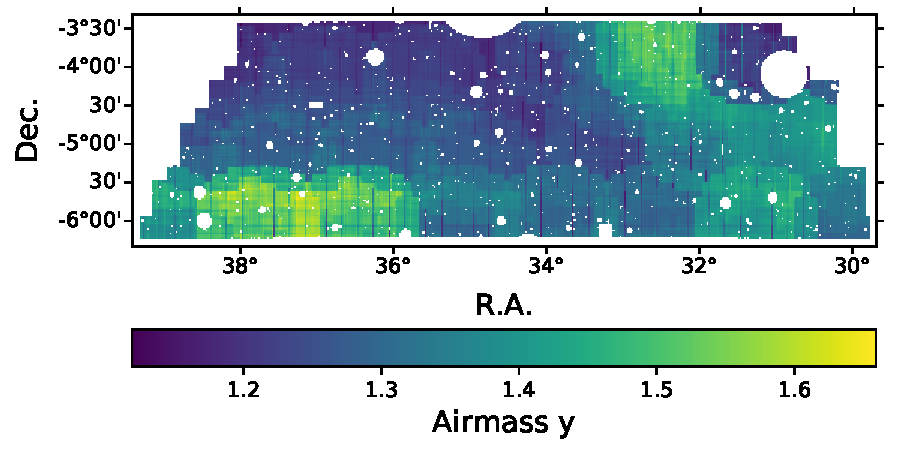
\includegraphics[width=0.49\textwidth]{figures/syst_airmass_y.pdf}
      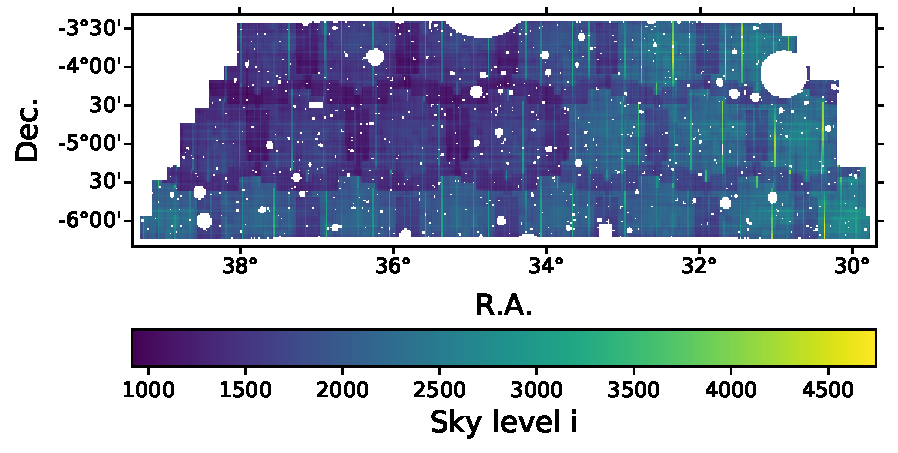
\includegraphics[width=0.49\textwidth]{figures/syst_skylevel_i.pdf}
      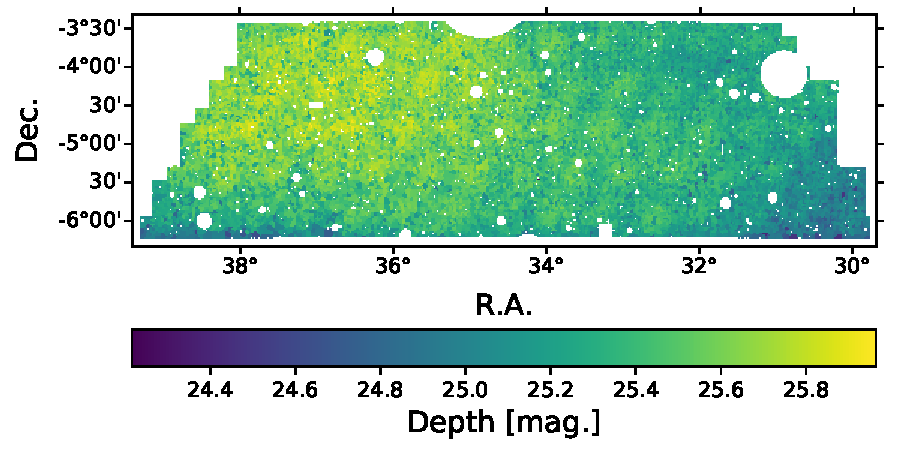
\includegraphics[width=0.49\textwidth]{figures/syst_depth.pdf}
      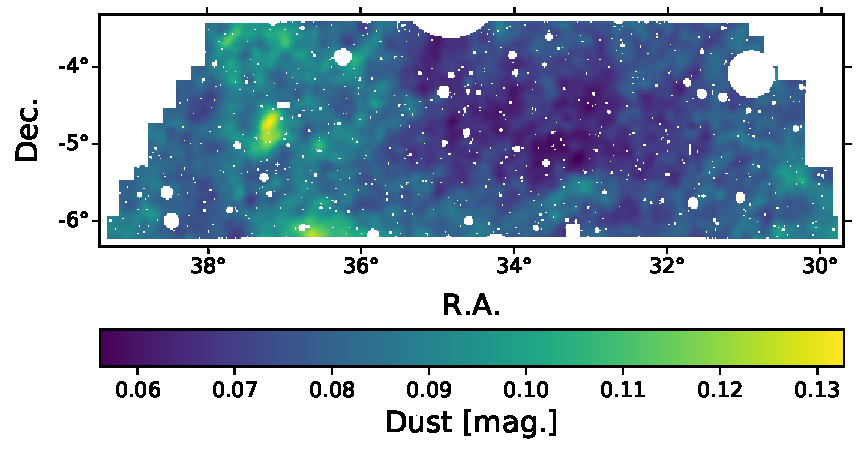
\includegraphics[width=0.49\textwidth]{figures/syst_dust.pdf}
      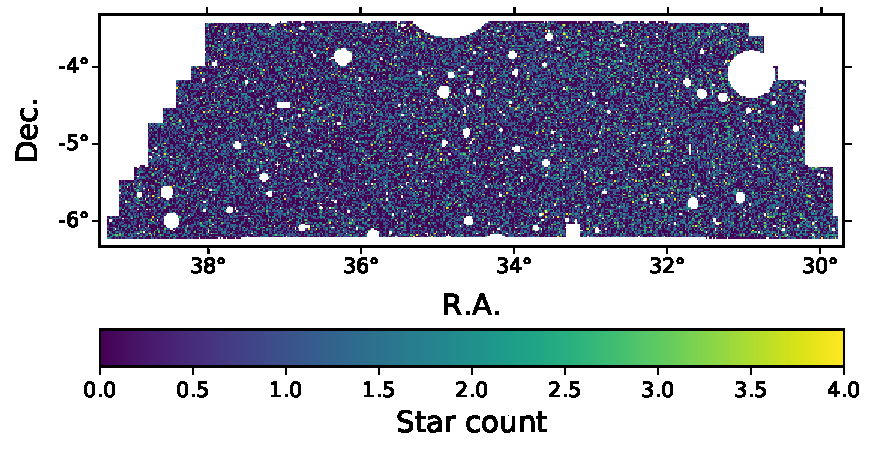
\includegraphics[width=0.49\textwidth]{figures/syst_star.pdf}
      \caption{Maps of different observational systematics that could cause an artificial modulation in the inferred galaxy overdensity. The maps correspond to the XMMLSS field, and were obtained as described in Section \ref{ssec:methods.syst}. From top to bottom and left to right, the different panels show maps of the seeing in the $g$, $i$ and $y$ bands, airmass in the $y$ band, sky level in the $i$ band, $10\sigma$ $i$-band depth, dust absorption and star density. We can visually appreciate the existing correlations between differnt systematics (e.g. seeing and airmass), which are automatically taken into account by the deprojection method described in Section \ref{ssec:methods.cell} and in \cite{2019MNRAS.484.4127A}.}
      \label{fig:sysmap}
    \end{figure}
    A number of astrophysical and observational systematic effects can affect the observed distribution of galaxies, and therefore may bias our inference of their clustering properties. To mitigate this effect we deproject maps of these systematics from our data, as described in Section \ref{ssec:methods.cell}. We generate maps of the most plausible sources of systematic variations in the galaxy number density:
    \begin{enumerate}
      \item {\bf Survey depth}: we estimate the $10\sigma$ survey depth in different directions using a method similar to that outlined in \cite{2018PASJ...70S..25M}. In a given sky pixel, we collect all galaxies with $i$-band {\tt cmodel} fluxes measured with a signal-to-noise ratio between 9 and 11 (i.e. $9\le{\tt icmodel\_flux}/{\tt icmodel\_flux\_err}\le11$), and compute the mean of their $i$-band  {\tt cmodel} magnitude. We verified that we obtain similar depth estimates using other methods (e.g. magnitude corresponding to $10$ times the mean flux error), and that the magnitude limit of our sample ($i<24.5$) is bright enough that little or no area is lost in any of the fields by imposing this cut.
      \item {\bf Dust extinction}: we make maps of dust absorption in each band using the data from \cite{1998ApJ...500..525S} projected onto the 6 HSC DR1 fields.
      \item {\bf Star contamination}: we produce a map of the number density of stars using all objects passing our sample cuts but classified as stars by the star-galaxy separator. As described in Section \ref{ssec:methods.cell}, the method used to remove the impact of this systematic is slightly different from the rest.
      \item {\bf Observing conditions}: the HSC DR1 provides metadata for each filter exposure, containing information about a number of observing conditions. We make coadded maps of these following a procedure similar to that described in \cite{2016ApJS..226...24L}. For each pixel in our map we gather all exposures that fully or partially overlap with it. For each quantity $Q$ in filter $f$, this allows us to build a list of values of $Q$ for each exposure\footnote{It is worth noting that we omit any exposure from CCD 9, since it was found to yield unreliable measurements and was never used in the HSC coadd images.}. We then compute the weighted mean of these values and assign the result to the pixel. The weights used to coadd different exposures consist of the product of the area overlap between pixel and exposure and an approximation of the weights used by the HSC pipeline to produce coadded images \cite{2018PASJ...70S...5B}. Since we do not have direct access to the latter, we used, as coadd weights, the inverse of the sky level of each exposure, which should be close to inverse-variance weighting. Following this procedure we produce maps of the following quantities: airmass, CCD temperature, seeing, point-spread function (PSF) ellipticity, exposure time, sky count level, root-mean square deviation of the sky count and number of visits.
    \end{enumerate}
    Figure \ref{fig:sysmap} shows examples of some of these maps.
    
    Note that an underlying assumption of this step is that the coadded mean of different exposures fully captures the connection between fluctuations in observing conditions and the artificial fluctuations they cause on the number counts. In general we could also consider other cumulants of the per-exposure distribution of observing condition values. As show below, we do not observe an important contamination from these systematics in our results, and therefore we leave this more thorough study for future work.

  \subsection{Redshift distributions}\label{ssec:methods.nz}
    \begin{figure}
      \centering
      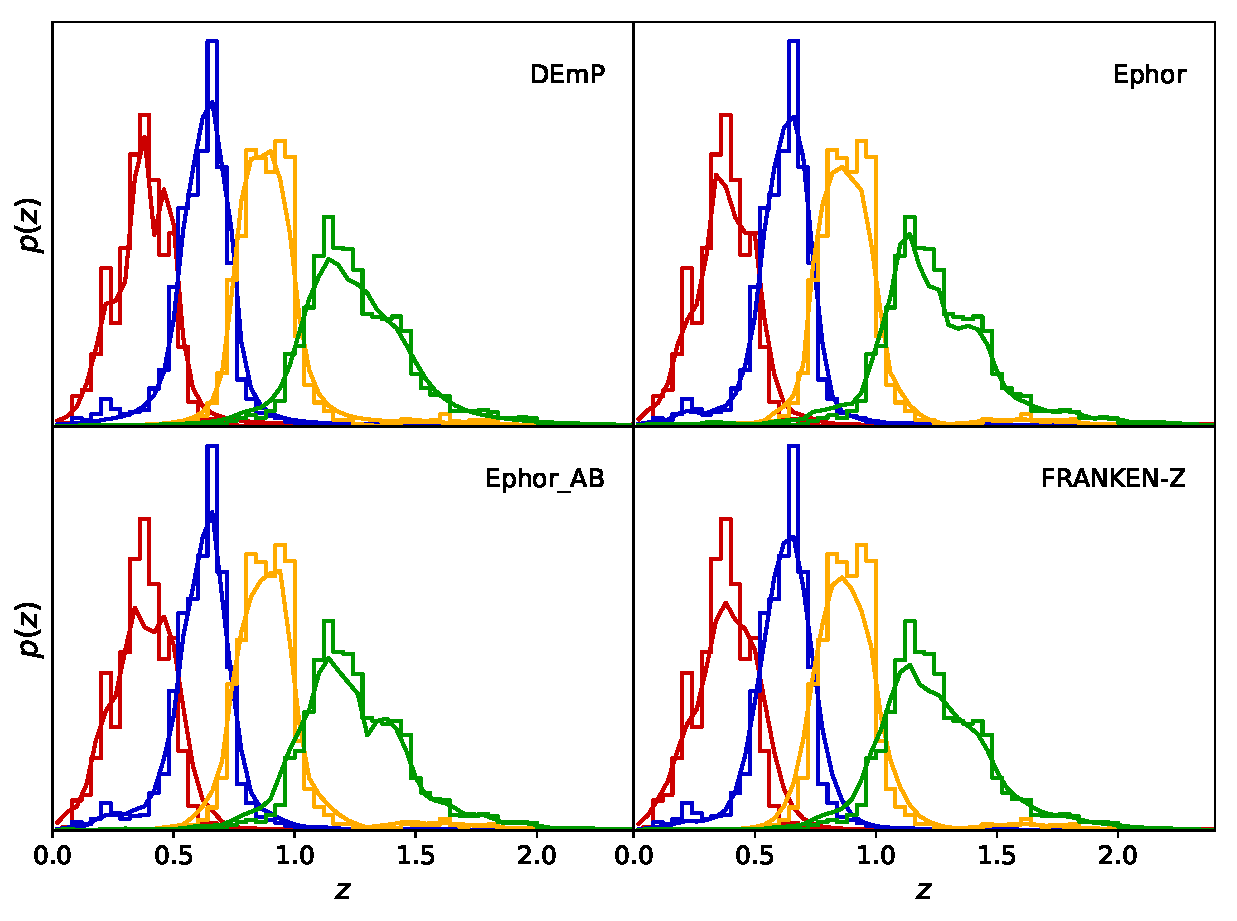
\includegraphics[width=0.9\textwidth]{figures/nzs.pdf}
      \caption{Redshift distributions used in this analysis. The histograms in each panel are the same, and correspond to the redshift distributions estimated from the COSMOS 30-band catalog. These are the fiducial redshift distributions used in our analysis. The solid curves in each panel show the stacked redshift distribution inferred by stacking the per-object photo-$z$ probability distributions obtained with the four alternative photo-$z$ codes explored here ({\tt DEmP}, {\tt Ephor}, {\tt Ephor\_AB} and {\tt Franken-Z} from left to right and top to bottom). The redshift distributions for the four different redshift bins listed in Table \ref{tab:bins_summary} are shown in red, blue orange and green respectively.}
      \label{fig:nzs}
    \end{figure}
    The underlying redshift distributions of our tomographic samples ($p^i(z)$ in Eq. \ref{eq:cell_gg_limber}) are a central component of the theory model used to infer astrophysical and cosmological parameters. Estimating redshift distributions for photometric samples is a non-trivial problem that has been studied extensively in the literature \todo{add a few citations}. We use two different methods to estimate $p^i(z)$.
    
    To estimate the fiducial redshift distributions used in our main analysis we make use of the COSMOS 30-band photometric catalog of \cite{2016ApJS..224...24L}. The idea is to use the high-fidelity photo-$z$ estimates in the COSMOS 30-band data as the truth, in which case one can estimate the redshift distribution by simply histogramming these redshifts with appropriate weights. These weights are calculated following the procedure described in \cite{2017MNRAS.465.1454H,2019PASJ...71...43H}, which we summarize here for completeness:
    \begin{enumerate}
      \item We first cross-match all objects in the COSMOS 30-band catalog with sources in the HSC COSMOS field that satisfy our sample cuts (see Section \ref{sec:data}). Matches are found as pairs of objects with an angular separation smaller than 1 arcsecond. All unmached objects in either catalog are discarded.
      \item For each object in the COSMOS 30-band data with a match on HSC, we find its $N_{\rm neigh}^{\rm COSMOS}=20$ nearest neighbours in the COSMOS 30-band sample within the 5-dimensional space of HSC apparent magnitudes $(g,r,i,z,y)$ using a Euclidean matrix. We record the distance in this space to the furthest neighbour.
      \item We then compute the number of HSC sources $N_{\rm neigh}^{\rm HSC}$ found within the same radius in magnitude space. The weight applied to the COSMOS 30-band object is then given by the ratio $N^{\rm HSC}_{\rm neigh}/N^{\rm COSMOS}_{\rm neigh}$ normalized by the total number of objects in each sample.
    \end{enumerate}
    There are a number of caveats associated with this method to estimate redshift distributions. First, the COSMOS 30-band photometric redshifts are not as good as a purely spectroscopic sample in terms of redshift accuracy and precision. Secondly, the small area covered by COSMOS may lead to sample variance uncertainties in the inferred redshift distributions that are difficult to quantify, particularly if the colour-redshift relation has an environmental dependence. Finally, the photo-$z$ codes used in HSC DR1 were trained on the COSMOS 30-band data, which could lead to circularity in the estimation of the redshift distributions.
    
    In order to study the dependence of our results on the method used to estimate the redshift distributions, we have also produced alternative estimates through a stacking approach. In this case, for a given photo-$z$ code, we produce and estimate of the redshift distribution of each tomographic bin by adding the photo-$z$ probability distributions of all objects in that bin. Following this procedure we generate 4 alternative estimates of $p^i(z)$ for the photo-$z$ codes {\tt demp}, {\tt ephor}, {\tt ephor\_ab} and {\tt frankenz} (see \cite{2018PASJ...70S...9T}) \an{What about NNPZ? I am asking because it is in the catalogs but I never got it to work as the pzs are all nan.}. The different redshift distributions for all tomographic bins and photo-$z$ methods are shown in Figure \ref{fig:nzs}. The different distributions are visually compatible with each other, although it must be noted that this is, to some extent, by construction, given that the different photo-$z$ codes were trained with the same data from the COSMOS 30-band catalog.

  \subsection{Angular power spectra}\label{ssec:methods.cell}
    We compute angular power spectra using a flat-sky pseudo-$C_\ell$ (PCL) algorithm \citep{2002ApJ...567....2H} using {\tt NaMaster}\footnote{\url{https://github.com/LSSTDESC/NaMaster}}. The reader is referred to the code's paper \cite{2019MNRAS.484.4127A} for a detailed description of the estimator, but we provide a brief summary here for completeness.
    
    In the absence of a sky mask, the flat-sky auto-power spectrum could be simply estimated Fourier transforming a given map $a_{\bf l}={\rm FT}[a(\nv),{\bf l}]$ (where ${\rm FT}$ denotes a Fourier transform operation, and ${\bf l}$ is a 2D wavenumber), and averaging its modulus squared over bins of $\ell\equiv|{\bf l}|$. In any practical situation, however, it will be desirable to apply weights on the map to e.g. downweight noisy areas or altogether remove pixels that haven't been observed. In this case the observed (``masked'') map is $\tilde{a}(\nv)=w(\nv)a(\nv)$, where $w(\nv)$ is a weight map. The Fourier coefficients of the observed map are therefore given by a convolution of the true Fourier coefficients with the Fourier transform of the maps, which therefore couples different $\ell$ modes in the original map. The result of using the na\"ive estimator of the power spectrum described above on the masked map is therefore a version of the true underlying power spectrum where different $\ell$s are coupled throught the so-called {\sl mode-coupling matrix} $M_{\ell\ell'}$:
    \begin{equation}
      \left\langle \tilde{C}^{ab}_\ell \right\rangle = \sum_{\ell'} M_{\ell\ell'}(w_a,w_b)\,C^{ab}_{\ell'}.
    \end{equation}
    Here, $\tilde{C}^{ab}_\ell$ is the power spectrum of two observed fields $\tilde{a}=w_a\,a$ and $\tilde{b}=w_b\,b$, and $C^{ab}_\ell$ is the true power spectrum. The PCL algorithm calculates the mode-coupling matrix analytically using the properties of the weight maps, and uses it to make an unbiased estimate of $C^{ab}_\ell$.
    
    The overdensity maps used are constructed as $\delta_{g,p}=N_p/(\bar{N}\,w_p)-1$, where $N_p$ is the number of sources in pixel $p$, $w_p$ is the survey mask described in Section \ref{ssec:methods.mask}, quantifying the unmasked area fraction in each pixel, and $\bar{N}$ is the mean number of sources per pixel, estimated as $\bar{N}=\sum_p N_p/\sum_p w_p$.
    
    An important aspect of power spectrum estimation that is particularly relevant for galaxy clustering studies is accounting for the effect of sky contaminants on the final summary statistic. In this analysis we have done so using a technique called ``template deprojection''. We start by compiling a list of maps of quantities that can potentially cause artificial perturbations in the observed number density of sources. These include all the quantities described in Section \ref{ssec:methods.syst}. The method then assumes that, at first order, these contaminants affect the observed galaxy overdensity linearly:
    \begin{equation}
      \delta_g^{\rm obs}(\nv) = \delta_g^{\rm true}(\nv) + A_{\rm syst}\,\Delta_{\rm syst}(\nv),
    \end{equation}
    where $\Delta_{\rm syst}$ is a template map of the fluctuation of a given contaminant around its mean across the survey footprint, and $A_{\rm syst}$ is an unknown linear factor. Template deprojection methods avoid systematic biases by  removing all modes from the observed maps that are common to any of the systematic template maps. In practice this is achieved by obtaining the best-fit value of $A_{\rm syst}$, subtracting the corresponding best-fit contaminant contribution from the maps and analytically accounting for the associated loss of modes when computing the angular power spectrum. Further details of this method can be found in \cite{2017MNRAS.465.1847E,2019MNRAS.484.4127A} . We must note that star contamination is a special type of contaminant, since it is an additive contribution to the observed galaxy number density $n_g$, not its overdensity. In the simplest scenario, a fraction $f$ of stars contribute to the observed galaxy density: $n_g^{\rm obs}=n^{\rm true}_g+f\,n_s$, where $n_s$ is the local number density of stars. A fluctuation in the star density around the mean $\Delta_s(\nv)=n_s(\nv)/\bar{n}_s-1$, therefore produces both a multiplicative and an additive effect on $\delta_g$:
    \begin{equation}
      \delta_g^{\rm obs}(\nv) = (1-F_s)\,\delta_g^{\rm true}(\nv)+F_s\,\Delta_s(\nv),
    \end{equation}
    where $F_s$ is the fraction of the sample made out of stars (i.e. $F_s\equiv f\bar{n}_s/(\bar{n}_g+f\bar{n}_s)$ with the notation above). The linear term is taken care of by the deprojection procedure, and we correct the final map of $\delta_g$ by a factor $1/(1-F_s)$, where we estimate $F_s$ from the HSC deep COSMOS field as described in section \todo{address this in Section \ref{sec:results}}.
    
    Finally, a noise bias term must be subtracted from all auto-power spectra. In the case of galaxy clustering, and assuming this noise is entirely due to Poisson shot noise, this can be done analytically as described in \cite{2019MNRAS.484.4127A}. In short, the noise power spectrum before mode-decoupling (i.e. before multiplying by the inverse mode-coupling matrix), can be calculated as:
    \begin{equation}
      \tilde{N}_\ell = \Omega_{\rm pix}\,\frac{\bar{w}}{\bar{N}},
    \end{equation}
    where $\bar{w}$ is the mean value of the survey mask across the map, $\bar{N}$ is the mean number density of sources per pixel, and $\Omega_{\rm pix}$ is the pixel area in units of steradians.
    
    \todo{More details may be needed on bandpower binning, bandpower windows, the exact procedure to compute $\tilde{N}_\ell$ etc.}

  \subsection{Covariance matrices}\label{ssec:methods.covar}
  
We use an analytical procedure to estimate the uncertainties of our measured power spectra, inspired in the methods used by \todo{cites}. As shown in \todo{cite}, the covariance matrix for large-scale structure data can be decomposed into a disconnected trispectrum part, essentially equivalent to the covariance of a Gaussian random field with the same power spectrum as the data, a connected part, caused by the non-Gaussian nature of the density field, and a super-sample covariance term (labelled SSC here), caused by the coherent shift in the amplitude of density fluctuations within the surveyed volume caused by long wavelength modes larger than the survey. 
    
    We estimate the Gaussian covariance of the pseudo-$C_\ell$ estimator as described in \todo{cite}. In the absence of any approximations, the covariance of the observed power spectra is given by
    \begin{equation}
      {\rm Cov}\left(\tilde{C}^{ab}_\ell,\tilde{C}^{cd}_{\ell'}\right)=\sum_{{\bf l}_1,{\bf l}_2} C^{ac}_{\ell_1}C^{bd}_{\ell_2}W^a_{{\bf l}{\bf l}_1}W^b_{{\bf l}{\bf l}_2}W^c_{{\bf l}'{\bf l}_1}W^d_{{\bf l}'{\bf l}_2} + C^{ad}_{\ell_1}C^{bc}_{\ell_2}W^a_{{\bf l}{\bf l}_1}W^b_{{\bf l}{\bf l}_2}W^c_{{\bf l}'{\bf l}_2}W^d_{{\bf l}'{\bf l}_1},
    \end{equation}
    where $W^x_{{\bf l}{\bf l}'}$ are coupling coefficients depending only on the mask of $x$ (see \todo{Cite} for further details). In the absence of further approximations, computing the covariance matrix would therefore imply solving a 4-dimensional integral for each pair $(\ell,\ell')$. I.e. an $O(\ell_{\rm max}^6$ operation which easily becomes computationally unfeasible. Since the coupling coefficients $W^x_{{\bf l}{\bf l}'}$ are usually highly peaked around ${\bf l}={\bf l}'$, we can proceed further by approximating the power spectra to be constant within the support of $W^x_{{\bf l},{\bf l}'}$. Effectively this implies approximating
    \begin{equation}
      C^{ac}_{\ell_1}C^{bd}_{\ell_2}\simeq C^{ac}_{(\ell}C^{bd}_{\ell')}\equiv\frac{1}{2}\left(C^{ac}_\ell C^{bd}_{\ell'}+C^{ac}_{\ell'} C^{bd}_\ell\right).
    \end{equation}
    This allows us to simplify the expression above significantly, becoming
    \begin{equation}
      {\rm Cov}\left(\tilde{C}^{ab}_\ell,\tilde{C}^{cd}_{\ell'}\right)=(2\ell'+1)^{-1}\left[C^{ac}_{(\ell}C^{bd}_{\ell')}M_{\ell\ell'}(w_aw_c,w_bw_d)+C^{ad}_{(\ell}C^{bc}_{\ell')}M_{\ell\ell'}(w_aw_d,w_bw_c)\right].
    \end{equation}
    Where $M_{\ell\ell'}$ are the mode-coupling matrices described in the previous section, except now are computed from the products of two masks. This approach has been shown by \todo{cite} to yield a very good approximation for the power spectrum covariance, fully accounting for the effects of mode coupling due to survey geometry. \todo{we did check this against gaussian simulations for this paper too. Do we want to show this? We'd need to regenerate those simulations and the corresponding plots.}
    
The second contribution to the total covariance matrix for galaxy clustering is caused by the connected part of the trispectrum, which accounts for mode-coupling due to the non-Gaussian nature of the density field. In our work we estimate this contribution using the halo model coupled with a halo occupation distribution. In general, this contribution is given by the angular projection of the three-dimensional trispectrum as
\begin{equation}
\mathrm{Cov}_{\mathrm{NG}}(C^{AB}_{\ell}, C^{CD}_{\ell'}) = \int \int \mathrm{d}\theta \;\mathrm{d}\chi \; \frac{q^{A}(\chi)q^{B}(\chi)q^{C}(\chi)q^{D}(\chi)}{\chi^{6}} \; T^{ABCD}(\sfrac{\ell}{\chi}, \sfrac{\ell'}{\chi}, \theta).
\end{equation}
Using the halo model, the connected part of the trispectrum $T^{ABCD}$ is given by (e.g. \cite{Takada:2013}):
\begin{equation}
T^{ABCD} = T^{ABCD, 1h} + (T^{ABCD, 2h}_{22} + T^{ABCD, 2h}_{13}) + T^{ABCD, 3h} + T^{ABCD, 4h},
\end{equation}
where
\begin{align}
&T^{ABCD, 1h}(\mathbf{k}_{1}, \mathbf{k}_{2}, \mathbf{k}_{3}, \mathbf{k}_{4}) = I^{0}_{ABCD}(k_{1}, k_{2}, k_{3}, k_{4}), \\
&T^{ABCD, 2h}_{22}(\mathbf{k}_{1}, \mathbf{k}_{2}, \mathbf{k}_{3}, \mathbf{k}_{4}) = P_{\mathrm{lin}}(k_{12})I^{1}_{AB}(k_{1}, k_{2})I^{1}_{CD}(k_{3}, k_{4}) + 2 \; \mathrm{perm.}, \\
&T^{ABCD, 2h}_{13}(\mathbf{k}_{1}, \mathbf{k}_{2}, \mathbf{k}_{3}, \mathbf{k}_{4}) = P_{\mathrm{lin}}(k_{1})I^{1}_{A}(k_{1})I^{1}_{BCD}(k_{2}, k_{3}, k_{4}) + 3 \; \mathrm{perm.}, \\
&T^{ABCD, 3h}(\mathbf{k}_{1}, \mathbf{k}_{2}, \mathbf{k}_{3}, \mathbf{k}_{4}) = B^{\mathrm{PT}}(\mathbf{k}_{1}, \mathbf{k}_{2}, \mathbf{k}_{34})I^{1}_{A}(k_{1})I^{1}_{B}(k_{2})I^{1}_{CD}(k_{3}, k_{4}) + 5 \; \mathrm{perm.}, \\
&T^{ABCD, 4h}(\mathbf{k}_{1}, \mathbf{k}_{2}, \mathbf{k}_{3}, \mathbf{k}_{4}) = T^{\mathrm{PT}}(\mathbf{k}_{1}, \mathbf{k}_{2}, \mathbf{k}_{3}, \mathbf{k}_{4})I^{1}_{A}(k_{1})I^{1}_{B}(k_{2})I^{1}_{C}(k_{3})I^{1}_{D}(k_{4}).
\end{align}
The quantities $B^{\mathrm{PT}}$ and $T^{\mathrm{PT}}$ denote the matter bi- and trispectrum respectively, as estimated using perturbation theory. The full expressions for these terms can be found in \cite{Takada:2013}. Finally, $I^{i}_{j}$ denotes the generic halo model integral, defined as (e.g. \cite{Krause:2017}):
\begin{align}
I^{i}_{A}(k) &= \int \mathrm{d}M \frac{\mathrm{d}n}{\mathrm{d}M} b_{A, i}(M) \langle \tilde{u}_{A}(k, M) \rangle, \\
I^{i}_{AB}(k, k') &= \int \mathrm{d}M \frac{\mathrm{d}n}{\mathrm{d}M} b_{A, i}(M) b_{B, i}(M) \langle \tilde{u}_{A}(k, M) \tilde{u}_{B}(k', M) \rangle, \\
I^{i}_{ABC}(k, k', k'') &= \int \mathrm{d}M \frac{\mathrm{d}n}{\mathrm{d}M} b_{A, i}(M) b_{B, i}(M) b_{C, i}(M) \langle \tilde{u}_{A}(k, M) \tilde{u}_{B}(k', M) \tilde{u}_{C}(k'', M) \rangle, \\
I^{i}_{ABCD}(k, k', k'', k''') &= \int \mathrm{d}M \frac{\mathrm{d}n}{\mathrm{d}M} b_{A, i}(M) b_{B, i}(M) b_{C, i}(M) b_{D, i}(M) \times \\ &\langle \tilde{u}_{A}(k, M) \tilde{u}_{B}(k', M) \tilde{u}_{C}(k'', M) \tilde{u}_{D}(k''', M) \rangle.
\end{align}
For simplicity, we follow \cite{Krause:2017} and approximate the 2- to 4-halo trispectrum as the linearily biased matter trispectrum and only include a probe-specific 1-halo trispectrum contribution.

Finally, we compute the super-sample covariance contribution following the treatment of \todo{cite}:
\begin{align}
\mathrm{Cov}_{\mathrm{SSC}}(C^{AB}_{\ell}, C^{CD}_{\ell'}) = \int & \mathrm{d}\chi \;\frac{q^{A}(\chi)q^{B}(\chi)q^{C}(\chi)q^{D}(\chi)}{\chi^{4}} \times \\ &\frac{\partial P_{AB}(\sfrac{\ell}{\chi}, z(\chi))}{\partial \delta_{b}}\frac{\partial P_{CD}(\sfrac{\ell'}{\chi}, z(\chi))}{\partial \delta_{b}}\sigma^{2}_{b}(z(\chi)).
\end{align}
The quantity $\frac{\partial P(k, z)}{\partial \delta_b}$ is the response of the matter power spectrum to a long-wavelength density fluctuation, which we estimate using the halo model and results from perturbation theory as\footnote{We note that we also consider an alternative SSC model, in which we estimate the response of the matter power spectrum as the linearly biased response for the matter field. We find our parameter constraints to be unaffected by this change.} (e.g. \cite{Krause:2017}):
\begin{align}
\frac{\partial P_{AB}(k, z)}{\partial \delta_{b}} &= \left( \frac{68}{21} - \frac{1}{3}\frac{\mathrm{d}\log{k^{3} P_{\mathrm{lin}}}(k, z)}{\mathrm{d}\log k} \right) I_{A}^{1}(k)I_{B}^{1}(k)P_{\mathrm{lin}}(k, z) + I_{AB}^{1}(k, k) \\ &- (b_{A} + b_{B})P_{AB}(k, z).
\end{align}
The quantity $b_{A}$ denotes the large-scale HOD bias for the $A$-th sample, computed as
\begin{equation}
b_{A}=\frac{1}{\bar{n}_{g, A}}\int \mathrm{d}M\,\frac{\mathrm{d}n}{\mathrm{d}M}b_{1}(M) \bar{N}_{c, A}(1+\bar{N}_{s, A}),
\end{equation}
and $\sigma_b^2(z)$ is the variance of the long wavelength mode over the survey footprint, given by
\begin{equation}
\sigma_b^2(z) = \int \frac{\mathrm{d}k_\perp^2}{(2\pi)^2}P_{\rm lin}(k_\perp,z)\left|W(k_\perp,z)\right|^2.
\end{equation}
Finally $W(k_\perp,z)$ denotes the Fourier transform of the survey footprint, which we approximate as a compact circle with an area matched to our data set:
\begin{equation}
W(k_\perp,z)=\frac{2 J_1(k_\perp\chi(z)\theta_s}{k_\perp \chi(z)\theta_s},\hspace{12pt} \theta_s={\rm arccos}(1-2f_{\rm sky}).
\end{equation}
 \todo{Describe how we coadd the power spectra of the different fields at some point}

\subsection{Parameter constraints}\label{ssec:methods.constr}
In order to derive constraints on HOD, cosmological and systematics parameters, we assume the joint likelihood of all auto- and cross-power spectra to be Gaussian 
\begin{align}
\mathscr{L}(D \vert \theta) = \frac{1}{[(2\pi)^{d}\det{C}]^{\sfrac{1}{2}}} e^{-\frac{1}{2}(\mathbf{C}^{\mathrm{obs}}_{\ell}-\mathbf{C}^{\mathrm{theor}}_{\ell})^{\mathrm{T}}C^{-1}(\mathbf{C}^{\mathrm{obs}}_{\ell}-\mathbf{C}^{\mathrm{theor}}_{\ell})}.
\label{eq:likelihood}
\end{align}
The quantity $C$ denotes the joint covariance matrix, which we estimate analytically for a cosmological model \todo{bla} and keep constant during parameter estimation.
We sample the likelihood in a Monte Carlo Markov Chain (MCMC) using the publicly available code \texttt{CosmoHammer} \cite{Akeret:2013}. For all sampled parameters, we assume flat, uniform priors. We sample the parameter set \todo{bla}. The sampled parameters are shown alongside their priors in Tab.~\ref{tab:params}.

\begin{table*}
\caption{Parameters varied in the MCMC with their respective priors and posterior means. The uncertainties denote the $68 \%$ c.l..} \label{tab:params}
\begin{center}
\begin{tabular}{ccc}
\hline\hline 
Parameter & Prior & Posterior mean\\ \hline \Tstrut                             
$M_{\mathrm{min}}$ & flat $\in [0., \,15.]$ & $- \pm -$ \\ 
$M_{\mathrm{min}, p}$ & flat $\in [-5., \,10.]$ & $- \pm -$ \\
$M_{0}$ & flat $\in [0., \,15.]$ & $- \pm -$ \\
$M_{0, p}$ & flat $\in [-5., \,10.]$ & $- \pm -$ \\
$M_{1}$ & flat $\in [0., \,15.]$ & $- \pm -$ \\ 
$M_{1, p}$ & flat $\in [-5., \,10.]$ & $- \pm -$ \\
$\Delta z_{i}$ & flat $\in [-0.2., \,0.2]$ & $- \pm -$ \\
\hline\hline 
\end{tabular}
\end{center}
\end{table*} 

\section{Results}\label{sec:results}
\subsection{Power spectra}
\subsection{Covariance matrix}
\subsection{Constraints on HOD parameters}
\subsubsection{Magnification bias}
In addition to intrinsic correlations between galaxy positions, there exist several additional effects affecting the observed clustering of galaxies. One of these is the magnification of distant sources due to the gravitational lensing effect of the intervening LSS. This effect is usually termed magnification bias. The statistical distribution of galaxies is mainly affected by magnification bias as it increases observed galaxy fluxes, thus allowing dim galaxies to pass survey selection thresholds. It has been shown that the clustering signal due to magnification bias can dominate over the intrinsic clustering signal for cross-correlations between widely separated redshift bins. As shown in Sec.~\ref{ssec:theory.mag}, the magnitude of the magnification bias signal crucially depends on the derivative of the galaxy number counts with respect to observed magnitude, $s(z)$. In order to obtain a data-driven model for magnification bias in our particular sample, we therefore estimate $s(z)$ from the observed number counts. Using linear least squares, we fit a fourth-order polynomial to the logarithm of the observed galaxy number counts $N(<m, z)$ in each of the four tomographic redshift bins considered in our analysis. We then determine $s(z)$ by taking the derivative of the best-fit function at the magnitude limit of our sample, i.e. $m_{i, \mathrm{lim}} = 24.5$. In addition to the WIDE HSC galaxy data used in this work, PDR1 also contains data from several deep patches, called DEEP and UDEEP. We repeat the above analysis on these galaxy samples to ensure the stability of our results. As an example, Fig.~\ref{fig:s-func-estimation} shows the observed number counts as a function of $i$-band magnitude for the lowest redshift in our fiducial WIDE sample alongside the derived best-fit function. In Fig.~\ref{fig:s-func-estimation}, we show the $s(z)$ functions derived as outlined above for HSC WIDE, DEEP and UDEEP. As can be seen from the Figure, the three estimates agree well with each other.

\begin{figure}
\begin{center}
\subfigure[Cumulative galaxy number counts as a function of $i$-band magnitude for lowest tomographic redshift bin.]{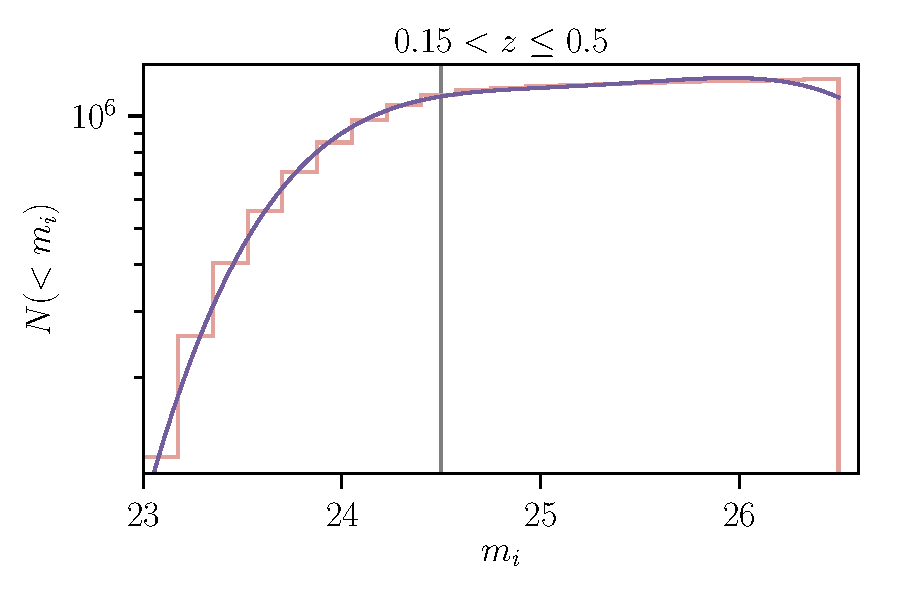
\includegraphics[width=0.49\textwidth]{figures/mag-dist-cumulative=True+fit-mmin=23-sample=WIDE-bin=0.pdf}}
\subfigure[Comparison of $s(z)$ (see Eq.~\ref{eq:s-func}) derived using WIDE, DEEP and UDEEP HSC galaxy samples.]{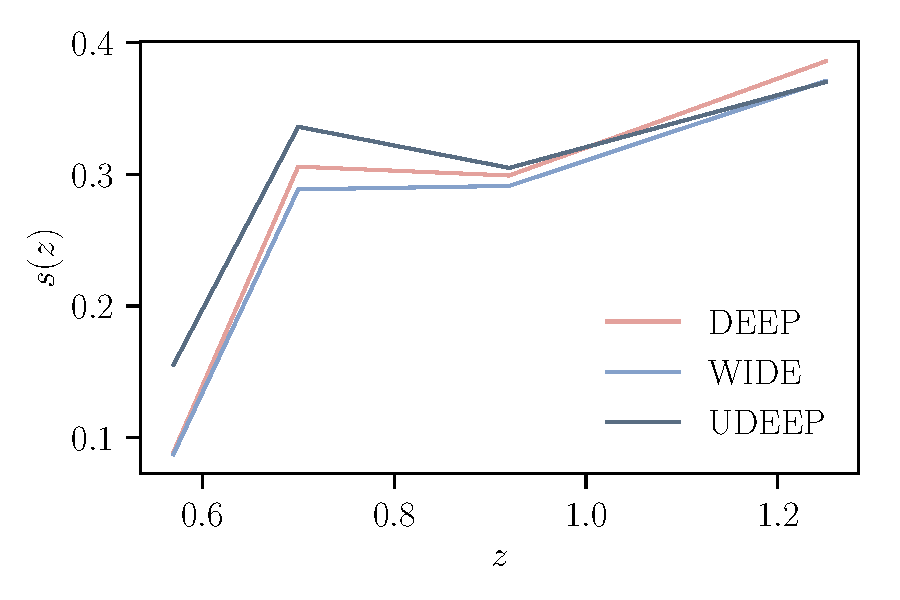
\includegraphics[width=0.49\textwidth]{figures/s-z-func-samples=WIDE-DEEP-UDEEP.pdf}} 
\caption{Illustration of data-driven estimation of $s(z)$ for galaxy sample used in our analysis.} 
\label{fig:s-func-estimation}
\end{center}
\end{figure}

Using the estimated $s(z)$, we can derive theoretical predictions for the angular galaxy power spectra in presence of magnification bias. In order to determine the best-fit model parameters accounting for magnification bias we run two different MCMCs: in the first case, we fix the magnification bias amplitude to the predictions from the empirically determined $s(z)$ function. In the second case we include an additional magnification bias parameter that scales the amplitude of the magnification kernel and we fit it alongside the other parameters.

\subsubsection{Interpretation of HOD results}

In order to understand the observed trend of decreasing $M_{\mathrm{min}}(z)$ and $M_{1}(z)$ with redshift, it would be ideal to look at the rest-frame properties of the galaxies considered in our analysis and how these change as a function of redshift. However, computing k-corrections and absolute magnitudes for broad-band photometric data can be challenging and we therefore choose and alternative approach. We cross-match galaxies passing our selection criteria within the HSC COSMOS field to galaxies also included in the COSMOS 30-band photometric catalog of \cite{2016ApJS..224...24L}. The COSMOS 30-band catalog contains, among others, absolute magnitudes in Subaru \texttt{B}-band, $M_{B}$, and Subaru \texttt{r+}-band, $M_{R}$. Using these quantities, we construct color-magnitude diagrams for all cross-matched galaxies. Fig.~\ref{fig:color-mag} shows the $M_{B}-M_{R}$ color as a function of $M_{R}$ magnitude for 10 equally spaced redshift bins in $z \in [0.15, 1.5]$\footnote{The galaxies are split into redshift bins according to COSMOS 30-band photometric redshifts. We note that we have repeated the analysis splitting the sample according to HSC \texttt{Ephor AB} photometric redshifts, finding consistent results.}. \an{We could also show the plot for the HSC splitting. What do you prefer?} In this diagram, red galaxies populate the high $M_{B}-M_{R}$ color, high $M_{R}$ magnitude plane, while blue galaxies tend to have lower $M_{B}-M_{R}$ and $M_{R}$. As can be seen from the figure, red galaxies increasingly drop-out of the high redshift samples. We can quantify this effect by computing the fraction of red galaxies in our sample as a function of redshift: we empirically determine the separation between the blue and red clouds (denoted by the solid lines in the figure) and compute the fraction of galaxies in the red cloud as $f_{R} = \sfrac{N_{R}}{(N_{R}+N_{B})}$, where $N_{R}$ denotes the number of galaxies above the separation line, while $N_{B}$ is the number of galaxies below the line. Consistent with the figure, we find decreasing $f_{R}$ as a function of redshift. 

This suggests that red galaxies increasingly drop-out of our sample due to the applied magnitude limit of $m_{\mathrm{lim}, i} < 24.5$.

%\begin{figure}
%\begin{center}
%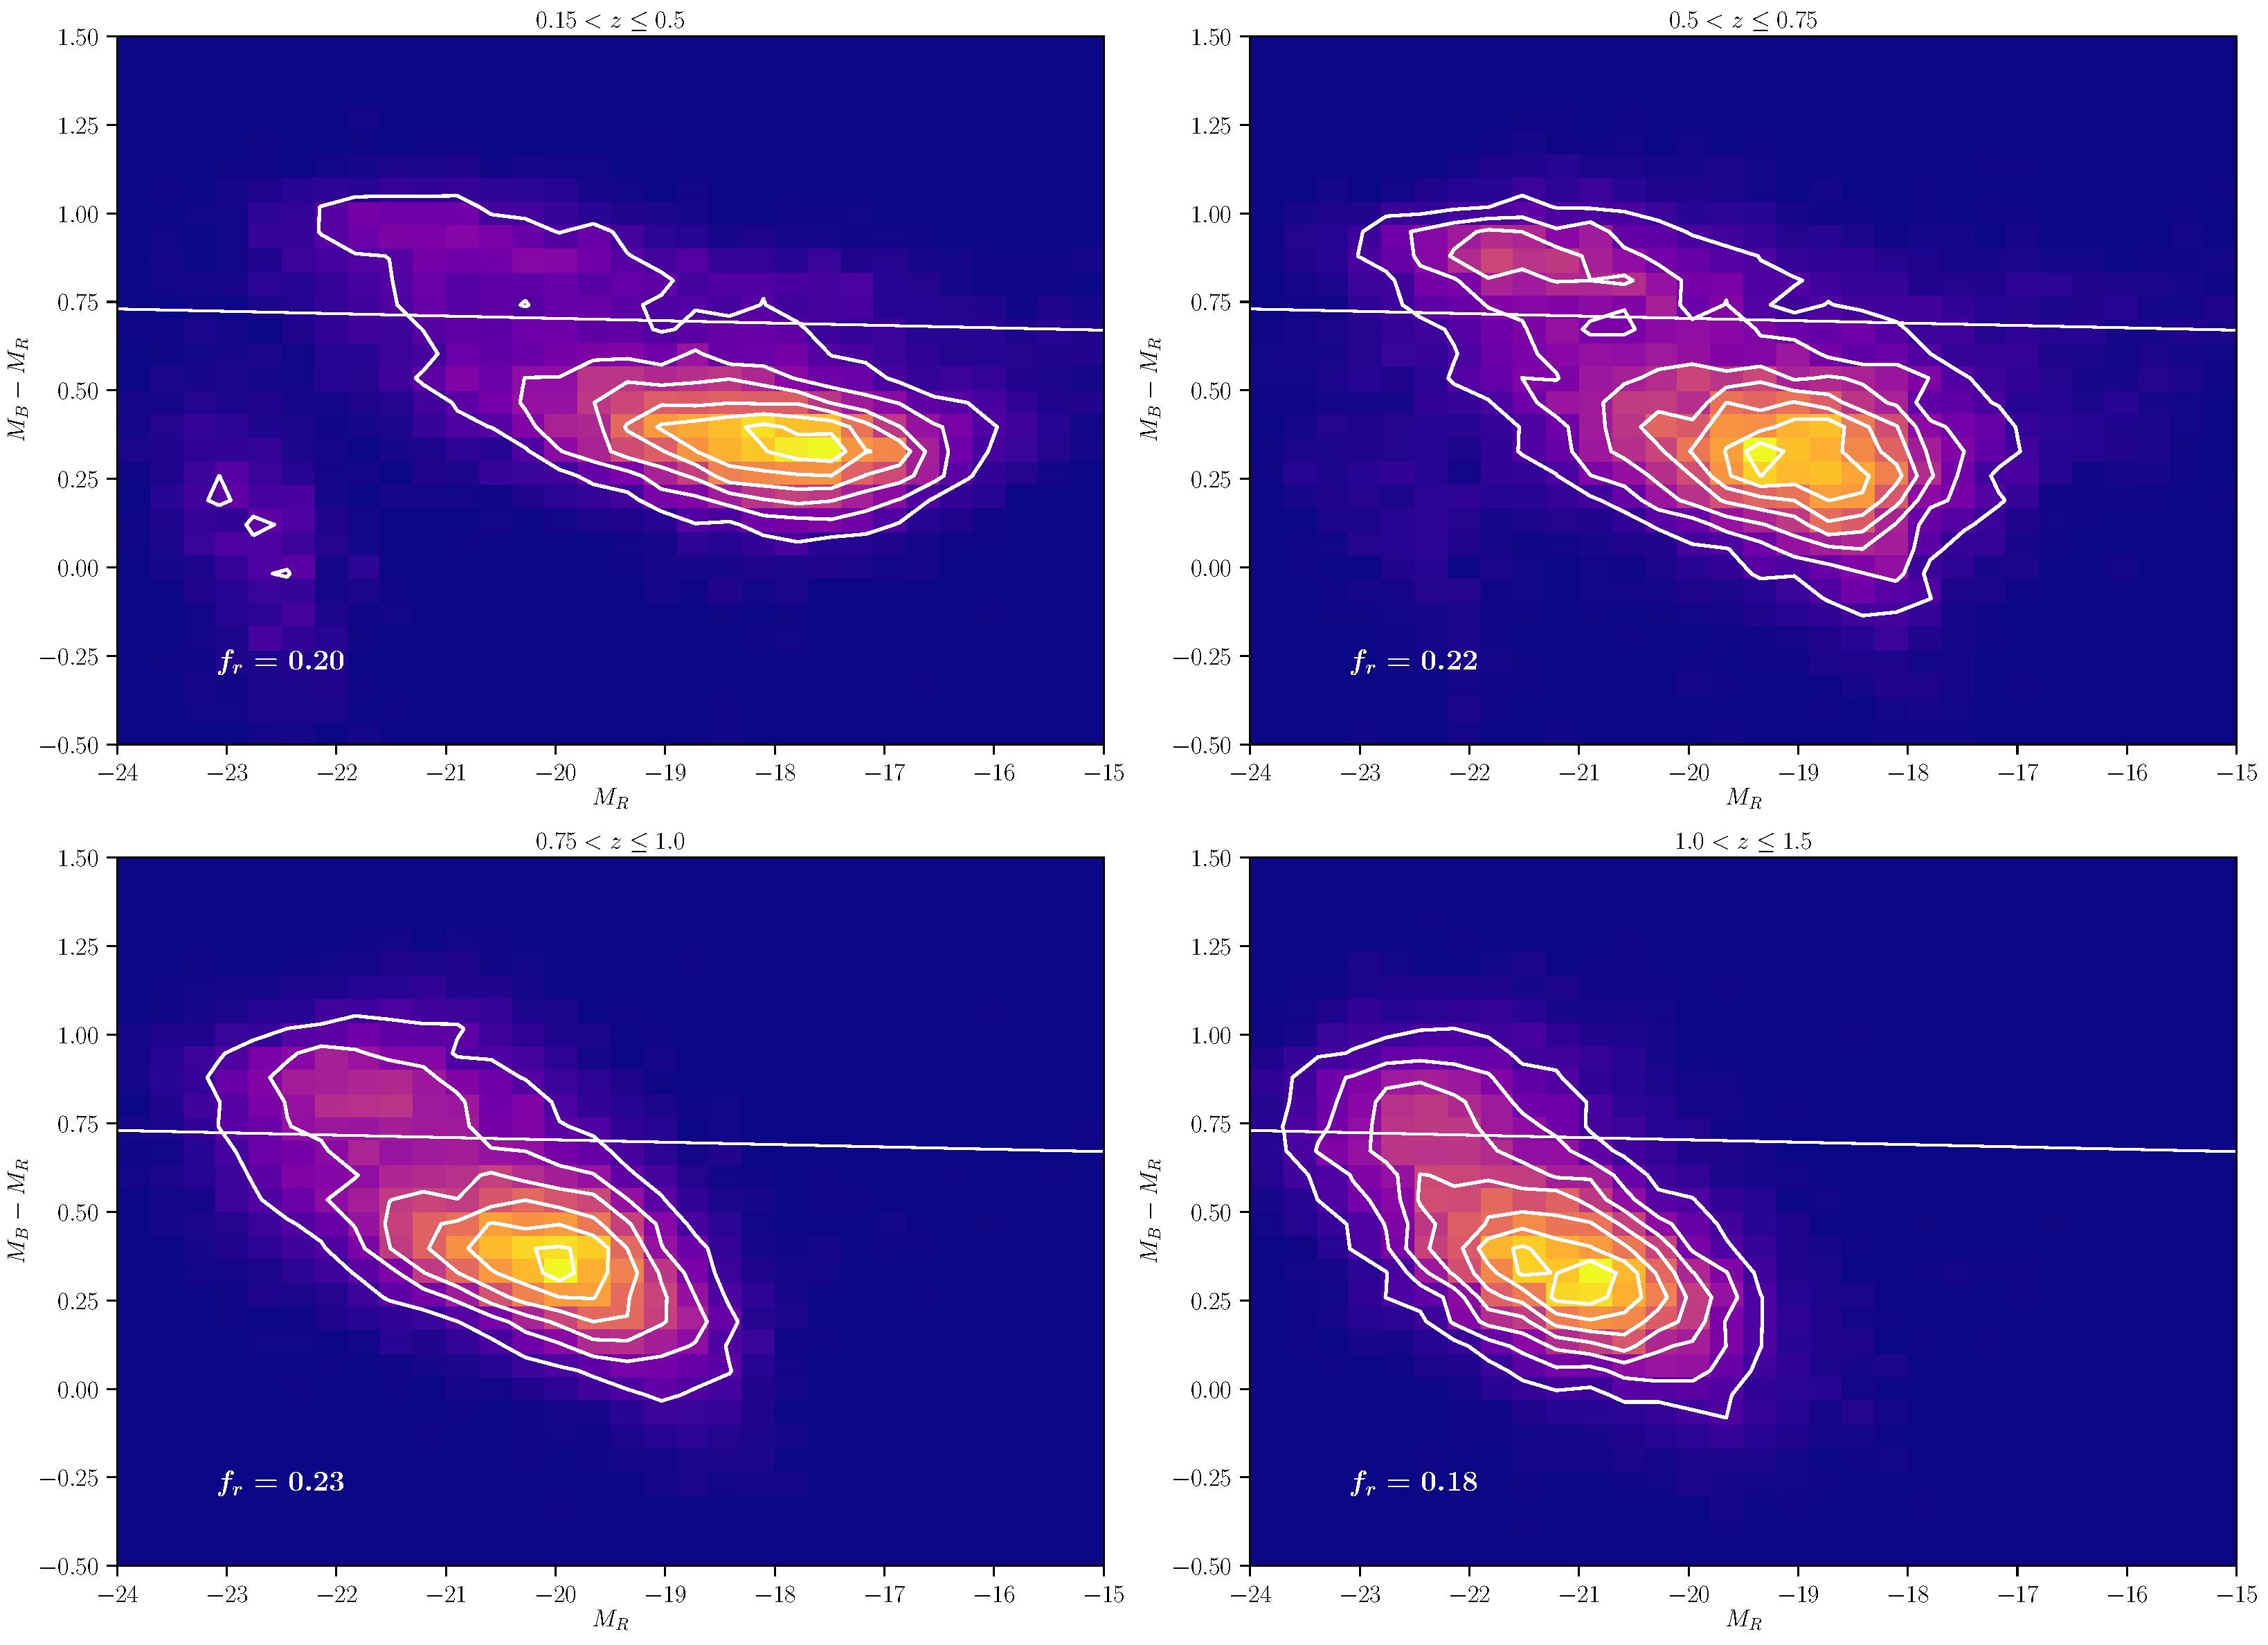
\includegraphics[scale=0.55]{figures/color-magnitude_cut=pz_best_eab_nbin=4_weights=True.pdf}
%\caption{Synopsis of the framework for integrated probe combination employed in this work.}
%\label{fig:color-mag}
%\end{center}
%\end{figure}

\begin{figure}
\begin{center}
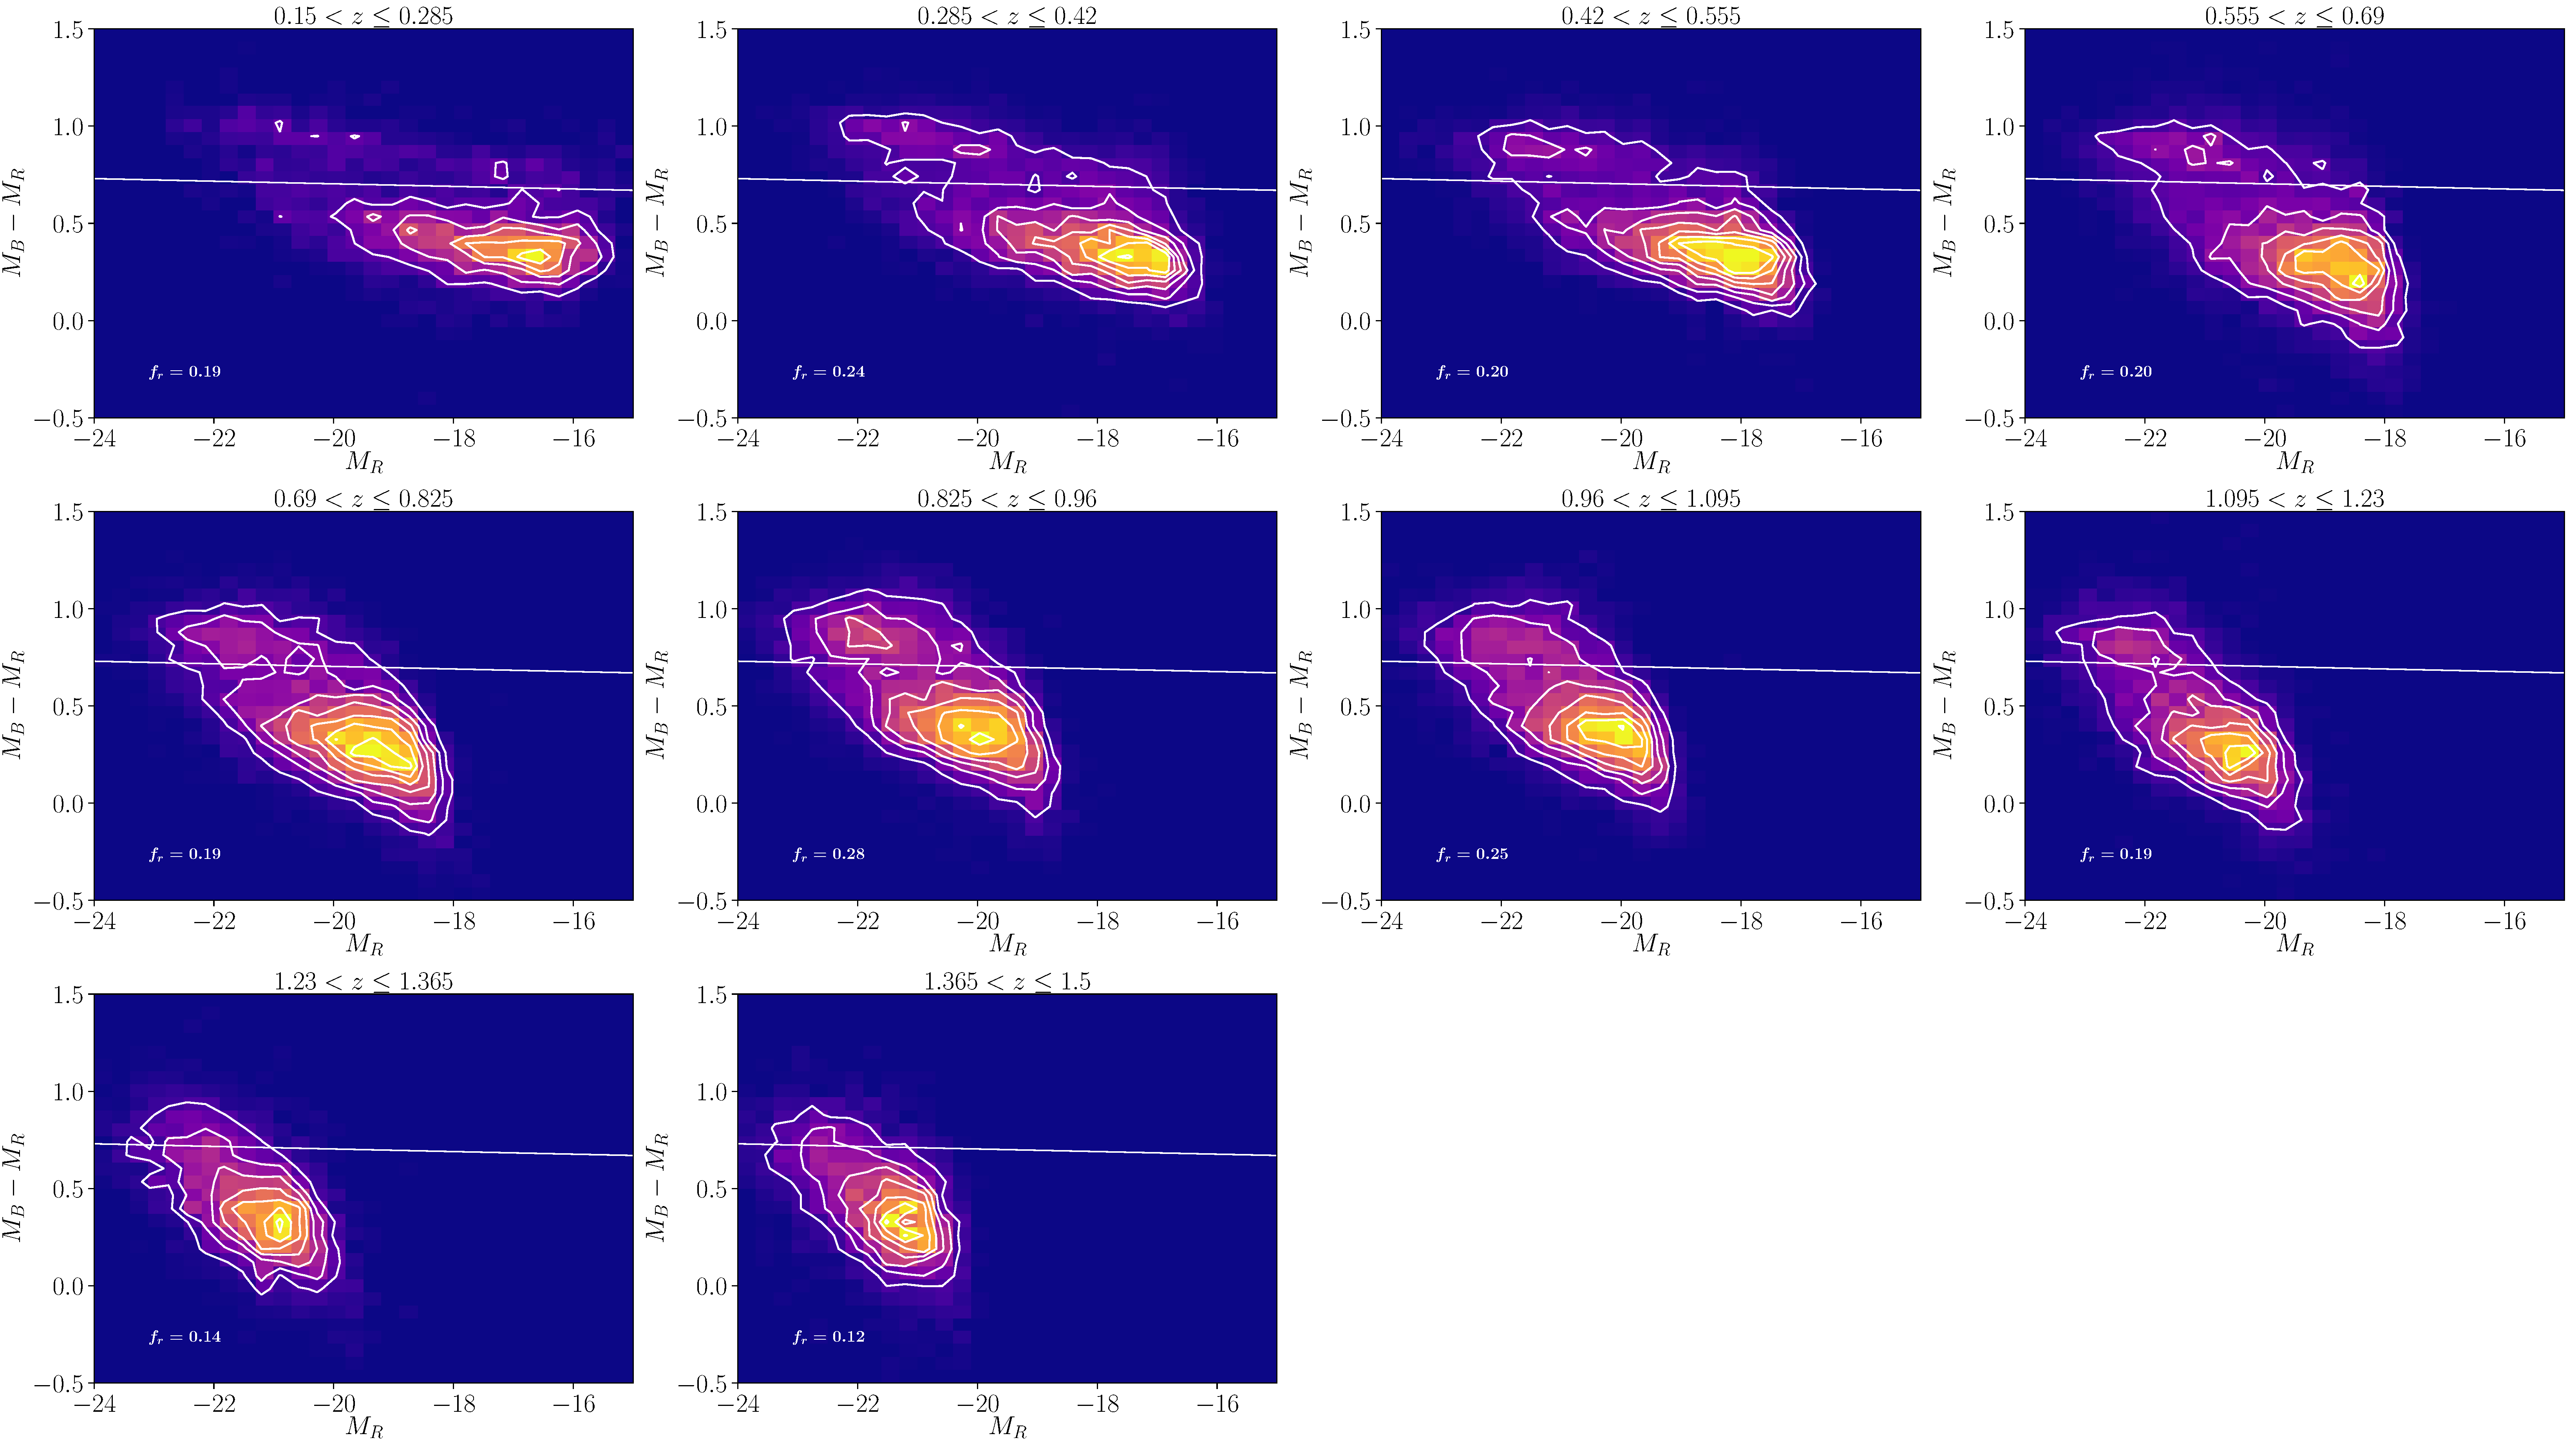
\includegraphics[width=0.95\textwidth]{figures/color-magnitude_cut=COSMOS30_nbin=10_weights=True.pdf}
\caption{Color-magnitude diagrams of COSMOS 30-band galaxies cross-matched to HSC galaxies passing our selection cuts for 10 tomographic redshift bins $z \in [0.15, 1.5]$.}
\label{fig:color-mag}
\end{center}
\end{figure}

  \todo{Things to discuss:}
  \begin{enumerate}
    \item Impact of systematics. Discuss star contamination in more detail (referenced above).
    \item Checks we've done: consistency between fields ($C_\ell$ and $N_{\rm gal}$), different masks, different levels of contaminant deprojection, different covariances.
    \item Effects of deprojection.
    \item Final contours.
    \item ...
  \end{enumerate}

\section{Discussion}\label{sec:discussion}
  \lipsum[9]

\acknowledgments

We thank the Backstreet Boys for useful comments and discussions.

\bibliography{bibliography}

\end{document}
